\documentclass[12pt,a4paper]{report}

% ---------------------------------------------------------
% Packages & Configuration
% ---------------------------------------------------------
\usepackage[utf8]{inputenc}
\usepackage[margin=1in,headheight=15pt]{geometry}
\usepackage{graphicx}
\usepackage{amsmath,amssymb}
\usepackage{booktabs}
\usepackage{array}
\usepackage{tabularx}
\usepackage{xltabular}
\usepackage{hyperref}
\usepackage{xcolor}
\usepackage{fancyhdr}
\usepackage{titlesec}
\usepackage{caption}
\usepackage{subcaption}
\usepackage{cite}
\usepackage{enumitem}
\usepackage{float}

\hypersetup{
    colorlinks=true,
    linkcolor=black,
    citecolor=black,
    urlcolor=blue!70!black
}

\pagestyle{fancy}
\fancyhf{}
\fancyhead[R]{\small \thepage}
\fancyhead[L]{\small \leftmark}
\renewcommand{\headrulewidth}{0.4pt}

\titleformat{\chapter}[display]
  {\normalfont\bfseries\Large}{\chaptertitlename\ \thechapter}{10pt}{\LARGE}
\titlespacing*{\chapter}{0pt}{-10pt}{15pt}

\begin{document}

% ---------------------------------------------------------
% Cover Page (Exact FAST Template Layout)
% ---------------------------------------------------------
\begin{titlepage}
    \centering
    \vspace*{0.5cm}
    
    {\huge \textbf{SilentAssist: Adaptive EEG-Based Assistive Home and Cognitive Support System}}\\[1.5cm]
    
    {\large Project Team}\\[0.3cm]
    {\large Abdul Haseeb Siddiqui \quad 23i-2654}\\[0.15cm]
    {\large Ali Farqleet \quad 22i-0579}\\[0.15cm]
    {\large Issa Sultan \quad 23i-2596}\\[1.5cm]
    
    {\large Session 2022--2026}\\[1.8cm]
    
    {\large Supervised by}\\[0.2cm]
    {\Large \textbf{Dr. Adil Majeed}}\\[1.8cm]
    
    \IfFileExists{figures/fast_logo.png}{\includegraphics[width=0.25\textwidth]{figures/fast_logo.png}\\[1.2cm]}{\vspace*{1.2cm}}
    
    {\large \textbf{Department of Artificial Intelligence and Data Science}}\\[0.2cm]
    {\large \textbf{FAST School of Computing}}\\[0.15cm]
    {\large \textbf{National University of Computer and Emerging Sciences}}\\[0.15cm]
    {\large \textbf{Islamabad, Pakistan}}\\[0.8cm]
    
    {\large \textbf{October, 2026}}
\end{titlepage}

% ---------------------------------------------------------
% Preliminary Pages (Roman Numerals)
% ---------------------------------------------------------
\pagenumbering{roman}
\setcounter{page}{1}

% Students' Submission
\newpage
\chapter*{Students' Submission}
\addcontentsline{toc}{chapter}{Students' Submission}

We certify that this report is submitted as the FYP-1 mid-report for the project titled \textbf{SilentAssist: Adaptive EEG-Based Assistive Home and Cognitive Support System}.\\[1.5cm]

\noindent
\begin{tabular}{@{}ll@{}}
\textbf{Student 1:} Abdul Haseeb Siddiqui (23i-2654) & \textbf{Signature:} \underline{\hspace{5.5cm}} \\[1.2cm]
\textbf{Student 2:} Ali Farqleet (22i-0579)          & \textbf{Signature:} \underline{\hspace{5.5cm}} \\[1.2cm]
\textbf{Student 3:} Issa Sultan (23i-2596)           & \textbf{Signature:} \underline{\hspace{5.5cm}} \\[1.5cm]
\end{tabular}

\vspace{0.8cm}
\noindent
\textbf{Supervisor:} Dr. Adil Majeed \\[0.2cm]
\textbf{Department:} Department of Artificial Intelligence and Data Science \\[0.2cm]
\textbf{Faculty:} FAST School of Computing, FAST-NUCES Islamabad \\[0.2cm]
\textbf{Submission Date:} October 2026

% Anti-Plagiarism Statement
\newpage
\chapter*{Anti-Plagiarism Statement}
\addcontentsline{toc}{chapter}{Anti-Plagiarism Statement}

The students certify that this report is their own authentic work and that all sources, literature, baseline architectures, and benchmark datasets used in preparing this report have been appropriately acknowledged and referenced.

We, Abdul Haseeb Siddiqui (23i-2654), Ali Farqleet (22i-0579), and Issa Sultan (23i-2596), confirm that no text, data, or design figures have been copied from external sources without explicit citation. In our experimental reproduction of the baseline neural network architecture, all reported empirical values represent our own original experimental executions and are honestly contrasted against published literature without claiming previous authors' results as our own.

% Authors' Declaration
\newpage
\chapter*{Authors' Declaration}
\addcontentsline{toc}{chapter}{Authors' Declaration}

We declare that the work documented in this report represents the work completed solely by the project team members, Abdul Haseeb Siddiqui (23i-2654), Ali Farqleet (22i-0579), and Issa Sultan (23i-2596), up to the FYP-1 mid-report stage under the supervision of Dr. Adil Majeed. All software implementations, neural decoding models, semantic reasoning engines, and evaluation pipelines represent our own authentic effort. External software libraries, computational frameworks, public benchmark datasets, and literature citations are disclosed separately and comprehensively in Chapter~8.

% Abstract
\newpage
\chapter*{Abstract}
\addcontentsline{toc}{chapter}{Abstract}

Severe neuromuscular paralysis resulting from conditions such as amyotrophic lateral sclerosis, tetraplegia, or spinal cord injury deprives individuals of their physical independence. Affected individuals often retain full cognitive awareness but lose the physical ability to operate basic domestic appliances such as lighting, fans, air conditioning, and media devices. Existing commercial assistive technologies fail to solve this problem effectively: physical switches require muscular movement that progressively degrades over time; eye-gaze tracking cameras cause rapid eye fatigue and suffer from accidental selections; and speech assistants cannot function when patients have speech impairments.

Brain-Computer Interfaces (BCIs) provide a direct communication pathway by measuring electrical brain activity using non-invasive electroencephalography (EEG) sensors placed on the scalp. When an individual imagines a movement, such as moving their hand or foot, the primary motor cortex generates detectable patterns known as Motor Imagery (MI). However, traditional motor-imagery systems suffer from three major shortcomings: they try to map dozens of complex thoughts to individual appliances, which rapidly exhausts the user; they lack awareness of domestic context; and they operate in an open loop where misclassifications trigger unintended actions that the patient cannot easily undo.

SilentAssist resolves these compounding challenges by introducing a closed-loop assistive system that unites neural decoding with semantic reasoning and automated error recovery. Motor intentions are decoded from 22-channel continuous EEG using a simple vocabulary of four universal navigation commands: imagining right-hand movement navigates forward, left-hand navigates backward, both feet selects an item, and tongue movement goes back to the previous menu. This design eliminates cognitive strain by allowing users to navigate through clear menus rather than memorizing complex motor tasks. To ground these commands in the real world, SilentAssist integrates the CogLign Knowledge Graph, which stores a semantic model of domestic rooms and devices using standard European Telecommunications Standards Institute (ETSI) and World Wide Web Consortium (W3C) smart-home ontologies. Actions are evaluated by a four-tier safety policy engine that protects patients from dangerous settings, such as extreme temperatures.

Most importantly, SilentAssist closes the control loop by monitoring frontocentral brain waves for Error-Related Potentials (ErrPs). When the brain recognizes an unintended system action, it naturally and involuntarily emits an error wave within 200 to 500 milliseconds. SilentAssist detects this signal in real time. If an error is recognized, the system immediately rolls back the appliance to its previous state, applies a penalty to the misclassified device in the knowledge graph, and automatically presents the next most probable option. At the midterm checkpoint, the team has successfully replicated the baseline deep neural network across nine subjects on a public benchmark dataset, diagnosed four structural limitations in the published literature, built a calibrated error-detection pipeline, developed an in-browser semantic reasoning engine, and delivered a complete offline prototype verified through automated testing pipelines.

% Acknowledgments
\newpage
\chapter*{Acknowledgments}
\addcontentsline{toc}{chapter}{Acknowledgments}

The project team expresses sincere gratitude to our supervisor, \textbf{Dr. Adil Majeed}, for his continuous technical guidance, academic mentorship, and constructive feedback throughout the design and implementation of this project. His expertise in machine learning, neuro-symbolic reasoning, and clinical assistive system design helped shape our research direction around credible, reproducible, and verifiable engineering deliverables.

We express our deepest appreciation to the faculty members, coordinators, and leadership of the \textbf{Department of Artificial Intelligence and Data Science}, within the \textbf{FAST School of Computing} at the \textbf{National University of Computer and Emerging Sciences (FAST-NUCES), Islamabad Campus}. Their rigorous academic standards, insightful evaluation feedback, and continuous support have provided us with the intellectual environment and academic guidance necessary to undertake this multidisciplinary engineering project.

Finally, we express our appreciation to the academic research community and the authors of the public neurotechnology benchmark datasets, including the Graz BCI laboratory for the BCI Competition IV Dataset 2a and the Horizon 2020 BNCI consortium for Dataset 013-2015. Their commitment to open science and publicly available clinical data made the reproducible evaluation of this project possible on standard computational hardware.

% Executive Summary
\newpage
\chapter*{Executive Summary}
\addcontentsline{toc}{chapter}{Executive Summary}

\textbf{Problem.} Millions of individuals worldwide live with severe physical paralysis caused by advanced neurodegenerative disorders, brainstem stroke, or spinal trauma. These individuals typically possess active, healthy cognitive faculties but are unable to control their physical surroundings, becoming entirely dependent on domestic caregivers for simple environmental alterations. While brain-computer interfaces offer a direct communication channel, traditional designs suffer from high cognitive fatigue, open-loop error propagation, and an absence of contextual safety boundaries.

\textbf{Project Vision.} SilentAssist aims to deliver an accessible, privacy-preserving, closed-loop assistive smart-home system. By combining deep graph neural decoding with client-side semantic knowledge representation and automated neurophysiological error correction, the system allows paralyzed users to manage domestic appliances independently, safely, and without mental exhaustion.

\textbf{Scope at FYP-1 Midterm.} The scope achieved at the midterm milestone includes:
\begin{enumerate}[leftmargin=1.5em]
    \item Replicating the baseline SFE-GAT graph neural network across all nine subjects of the public BCI Competition IV-2a dataset under strict subject-dependent evaluation.
    \item Developing a calibrated Error-Related Potential detection pipeline using shrinkage Linear Discriminant Analysis and Platt scaling on the BNCI 013-2015 benchmark dataset.
    \item Building the client-side CogLign Knowledge Graph using ETSI SAREF and W3C BOT ontologies with an in-browser SPARQL query engine.
    \item Implementing a four-tier decision-theoretic policy engine that enforces thermal and electrical safety boundaries.
    \item Constructing a fully functional, zero-build offline web prototype featuring high-contrast accessible navigation, spoken audio feedback, a caregiver supervision dashboard, and a tamper-evident audit ledger based on SHA-256 cryptographic hashing.
    \item Establishing an automated Continuous Integration pipeline on GitHub Actions with five quality gates enforcing unit testing, browser testing, and mathematical parity.
\end{enumerate}

\textbf{Research Findings.} Our experimental replication of the SFE-GAT architecture yielded an average subject-dependent classification accuracy of 35.68\% across the nine subjects on held-out evaluation trials, in contrast to the 77.70\% reported in the original paper. Rather than concealing this difference, our team conducted a thorough diagnostic audit and isolated four structural root causes: graph auto-encoder gradient starvation caused by pure cross-entropy loss, unnormalized power spectral density node features, severe inter-session power drift, and model overfitting. On the error-detection pipeline, our model achieved a cross-session balanced accuracy of 71.0\% and an area under the ROC curve of 0.780, demonstrating that involuntary brain potentials can reliably automate error recovery.

\textbf{Implementation and Testing Status.} All six core modules are fully implemented and demonstrable. The client interface runs completely offline directly from local disk files without requiring remote servers or web daemons. The codebase is verified by 234 automated tests across Python, Node.js, and headless browser environments, achieving mathematical parity between PyTorch neural network weights and browser JavaScript calculations within an absolute tolerance of $9.77 \times 10^{-15}$.

\textbf{Risks and Remaining Work.} The remaining work for FYP-1 Final focuses on refining the neural network architecture by introducing logarithmic power normalization and auxiliary graph auto-encoder reconstruction loss to close the replication gap, followed by leave-one-subject-out cross-validation.

% Table of Contents, Figures, Tables
\newpage
\tableofcontents
\listoffigures
\listoftables

% List of Abbreviations
\newpage
\chapter*{List of Abbreviations}
\addcontentsline{toc}{chapter}{List of Abbreviations}

\begin{tabularx}{\textwidth}{@{}p{3.0cm} X@{}}
\toprule
\textbf{Abbreviation} & \textbf{Full Term / Definition} \\
\midrule
ALS & Amyotrophic Lateral Sclerosis \\
API & Application Programming Interface \\
AUC & Area Under the Receiver Operating Characteristic Curve \\
BA & Balanced Accuracy \\
BCI & Brain-Computer Interface \\
BOT & Building Topology Ontology (W3C Linked Building Data Standard) \\
CAR & Common Average Reference \\
CI/CD & Continuous Integration / Continuous Deployment \\
CSP & Common Spatial Pattern \\
DSP & Digital Signal Processing \\
EEG & Electroencephalography \\
ERD & Entity-Relationship Diagram \\
ERN & Error-Related Negativity \\
ErrP & Error-Related Potential \\
FBCSP & Filter Bank Common Spatial Pattern \\
FR & Functional Requirement \\
FYP & Final Year Project \\
GAE & Graph Auto-Encoder \\
GATv2 & Graph Attention Network version 2 \\
GNN & Graph Neural Network \\
KG & Knowledge Graph \\
LDA & Linear Discriminant Analysis \\
LOSO & Leave-One-Subject-Out Cross-Validation \\
MI & Motor Imagery \\
NFR & Non-Functional Requirement \\
Pe & Error Positivity \\
PLV & Phase Locking Value \\
PSD & Power Spectral Density \\
RDF & Resource Description Framework \\
SAREF & Smart Applications REFerence Ontology (ETSI TS 103 264) \\
SCI & Spinal Cord Injury \\
SFE-GAT & Structure-Feature Evolution Graph Attention Network \\
SPARQL & SPARQL Protocol and RDF Query Language \\
SVM & Support Vector Machine \\
UML & Unified Modeling Language \\
WCAG & Web Content Accessibility Guidelines \\
\bottomrule
\end{tabularx}

% ---------------------------------------------------------
% CHAPTER 1: INTRODUCTION AND PROJECT VISION
% ---------------------------------------------------------
\newpage
\pagenumbering{arabic}
\setcounter{page}{1}

\chapter{Introduction and Project Vision}

\section{Project Overview}
SilentAssist is an adaptive, closed-loop Brain-Computer Interface designed to restore domestic independence for individuals living with profound physical paralysis. The system is specifically engineered for patients suffering from advanced neuromuscular conditions such as amyotrophic lateral sclerosis, severe tetraplegia, or cervical spinal cord injury. These individuals frequently retain intact cognitive, intellectual, and sensory faculties, yet they are trapped inside their own bodies without the ability to move their arms, speak clearly, or operate household switches.

The core premise of SilentAssist is to translate non-invasive electroencephalographic signals recorded from the scalp into reliable environmental control actions, such as turning on lights, adjusting fans, setting comfortable room temperatures, and switching media entertainment. Rather than requiring the user to master complex, exhausting mental tasks for every single appliance, SilentAssist uses four universal motor-imagery commands that allow the patient to navigate a structured, clear menu: imagining right-hand movement moves forward, imagining left-hand movement moves backward, imagining foot movement selects an item, and imagining tongue movement returns to the previous screen.

To ensure that the decoded thoughts translate into safe and meaningful actions, the system combines neural signal processing with a client-side semantic knowledge graph. This knowledge graph understands the physical arrangement of the domestic environment, active appliances, and current room states. Furthermore, the system incorporates an automated Error-Related Potential detection pipeline. If the neural decoder makes an error and selects the wrong appliance, the patient's brain naturally produces an involuntary error potential. SilentAssist detects this signal immediately, cancels the unintended action before it causes frustration, and restores the previous appliance state. The entire client application is built to run completely offline on standard web browsers, ensuring absolute privacy, zero network latency, and complete dependability within home healthcare environments.

\section{Problem Statement}
Severe physical paralysis represents one of the most isolating and challenging conditions in modern clinical neurology. When individuals suffer from advanced neuromuscular diseases such as Amyotrophic Lateral Sclerosis, bilateral brainstem stroke, or high-cervical spinal trauma, their somatic motor pathways become severely interrupted. In this locked-in state, a person's cognitive faculties, intellect, long-term memory, and emotional desires remain fully alert and active, but the neurological pathways needed to control skeletal muscles are lost. In daily domestic life, this creates an agonizing struggle: a patient lying in bed cannot switch on a reading lamp, cannot modulate a fan during sudden heat, cannot alter an uncomfortable room temperature, and cannot operate entertainment devices without summoning a caregiver. Every single domestic interaction requires vocalizing or waiting for external help, creating deep psychological frustration, diminishing personal dignity, and reinforcing a sense of helplessness.

Existing assistive technologies fail to solve this problem effectively in real-world domestic settings. Physical switches, such as mechanical push-buttons or sip-and-puff straws, rely entirely upon residual muscular movements. In degenerative disorders like ALS, motor neurons progressively deteriorate, rendering physical switches completely useless over time. Eye-gaze tracking cameras, which use infrared illumination to calculate pupil gaze coordinates, provide an alternative but introduce severe clinical drawbacks. Using an eye-tracker requires continuous, focused muscular control of the extraocular muscles. Clinical studies consistently report that motor-impaired patients experience extreme ocular fatigue, dry eyes, burning sensations, and headaches within thirty to forty-five minutes of continuous use. Furthermore, patients with drooping eyelids (ptosis) or involuntary eye tremors (nystagmus) cannot use eye-trackers reliably. Most importantly, eye-trackers suffer from the problem of distinguishing deliberate fixations from accidental visual glances, leading to frequent unintentional selections. Commercial voice-controlled assistants, such as Amazon Alexa or Google Home, are entirely unviable because progressive neuromuscular diseases weaken the vocal cords and facial muscles, causing speech impairment (dysarthria) or complete loss of speech (aphonia). Additionally, commercial speech assistants continuously transmit private domestic audio to third-party cloud servers, creating unacceptable privacy and security hazards in vulnerable home healthcare settings.

Non-invasive Brain-Computer Interfaces based on motor imagery offer a promising alternative by capturing electrical brain waves directly from the scalp, bypassing damaged peripheral nerves. However, conventional assistive BCIs remain confined to academic research laboratories because of three structural shortcomings. First, traditional systems attempt to assign a distinct mental thought to every individual household appliance. For example, a system might ask a patient to imagine moving their right hand to turn on a lamp, their left hand for a fan, their right foot for a television, their left foot for a radio, and their tongue for an air conditioner. Because electrical signals recorded through the scalp have a very low signal-to-noise ratio and are smeared by the skull, asking a patient to reliably sustain dozens of distinct mental rehearsals causes rapid mental burnout and high error rates. Second, conventional neural decoders operate completely without context: they emit raw numerical classifications without any awareness of where the patient is located, what appliances exist in that room, or whether a command is physically safe.

The most severe flaw of existing assistive BCIs is their open-loop operation. In non-invasive EEG systems, classification errors are statistically unavoidable due to electrode impedance shifts, muscle artifacts, and natural mental drift. When an open-loop BCI makes an error, the incorrect command is immediately executed on the physical appliance. A paralyzed patient who cannot move or speak has no easy way to undo this mistake. To correct a single accidental selection, the patient is forced to struggle through several additional minutes of mental navigation. This creates cascading errors, intense psychological frustration, and ultimately leads patients to abandon assistive technologies.

To overcome these compounding challenges, an assistive system must fundamentally rethink the interaction loop. It must eliminate cognitive strain by using a minimal, intuitive set of navigation primitives; it must ground neural intents within an intelligent domestic knowledge graph that understands rooms, devices, and safety rules; and above all, it must close the loop by automatically detecting the brain's natural, involuntary reaction to errors and reversing mistakes without requiring conscious patient struggle.

\section{Problem Context and Motivation}
In many developing healthcare ecosystems, including Pakistan, formal institutional care facilities for locked-in patients are either unavailable or financially prohibitive for average households. Consequently, the burden of full-time patient care falls almost entirely upon family members. In domestic settings, caregivers must balance personal employment with round-the-clock physical assistance, leading to emotional stress and physical exhaustion. Providing paralyzed individuals with an independent method to manage their personal environment directly enhances their sense of agency and reduces caregiver strain.

Recent advances in neural signal processing and graph neural networks offer promising tools to improve EEG classification accuracy. Functional brain connectivity can be modeled as a mathematical graph, where EEG electrodes represent nodes and statistical phase synchronization between brain regions represents edges. At the same time, semantic web ontologies provide standardized frameworks to describe domestic spaces, devices, and operational states. By unifying continuous graph neural networks with discrete symbolic knowledge graphs and closing the loop through neurophysiological error detection, SilentAssist bridges the gap between academic neurotechnology research and real-world domestic viability.

\sectionsection{Project Vision}
The vision of SilentAssist is to establish an accessible, privacy-preserving, and fatigue-free assistive control ecosystem. The project aims to prove that non-invasive electroencephalography, when thoughtfully combined with client-side semantic reasoning and closed-loop error correction, can provide safe, dependable, and dignified environmental autonomy to individuals living with severe physical paralysis, without requiring expensive specialized hardware or cloud connectivity.

\sectionsection{Project Objectives}
The concrete objectives established for the project are:
\begin{enumerate}[leftmargin=1.5em]
    \item Replicate and evaluate the Structure-Feature Evolution Graph Attention Network (SFE-GAT) baseline across all nine subjects of the BCI Competition IV-2a benchmark dataset under strict subject-dependent evaluation, identifying empirical limitations and root causes.
    \item Implement an automated Error-Related Potential signal processing and classification pipeline on the BNCI 013-2015 benchmark dataset, achieving cross-session balanced accuracy above 65\% and establishing a cost-theoretic decision threshold for automated state rollbacks.
    \item Construct the CogLign Knowledge Graph using standard ETSI SAREF and W3C BOT ontologies, supported by a client-side SPARQL 1.1 query engine that resolves contextual device queries in under five milliseconds directly within the browser.
    \item Develop a four-tier decision-theoretic safety policy engine that combines neural decoder confidence with knowledge graph semantic validity, preventing hazardous appliance operations and managing caregiver approvals.
    \item Deliver an offline-first, zero-build assistive web prototype that implements high-contrast navigation carousels, spoken audio feedback, a caregiver supervision hub, and a tamper-evident audit ledger using cryptographic hashing.
    \item Deploy an automated Continuous Integration pipeline on GitHub Actions that validates code syntax, executes unit tests, performs headless browser testing, and proves mathematical parity between Python models and browser execution.
\end{enumerate}

\section{Project Scope}
The scope of SilentAssist is carefully bounded between the deliverables completed for the FYP-1 Midterm evaluation and the extended goals planned for subsequent iterations.

\subsection{In-Scope (Midterm Deliverables)}
The functionality completed and demonstrated for the midterm evaluation includes:
\begin{itemize}[leftmargin=1.5em]
    \item Universal four-token motor imagery navigation vocabulary mapping right-hand imagination to forward navigation, left-hand to backward navigation, foot movement to item selection, and tongue movement to menu exit.
    \item Twenty-two channel digital signal processing extracting Phase Locking Value functional connectivity matrices and eight-band Welch Power Spectral Density node features.
    \item Complete subject-dependent replication of the SFE-GAT deep neural network across all nine subjects of the BCI Competition IV-2a dataset, accompanied by an audited analysis of reproduction discrepancies.
    \item Client-side forward pass inference engine that executes the graph attention network inside browser JavaScript, matching PyTorch floating-point outputs within an error of $9.77 \times 10^{-15}$.
    \item Single-trial Error-Related Potential classification pipeline using causal Butterworth filtering, shrinkage Linear Discriminant Analysis, Platt probability calibration, and Bayesian cost thresholding.
    \item In-browser Resource Description Framework triplestore implementing the CogLign Knowledge Graph, supporting materialization and SPARQL 1.1 query resolution.
    \item Four-tier safety policy engine evaluating composite confidence and routing high-risk operations, such as extreme thermal adjustments, to a caregiver approval queue.
    \item Accessible web application running completely offline from local disk files, featuring six patient navigation screens, synthesized speech feedback, a caregiver dashboard, and a SHA-256 hash-chained audit ledger.
    \item Automated GitHub Actions continuous integration workflow enforcing five verification gates on every code commit.
\end{itemize}

\subsection{Out-of-Scope (Deferred Functionality)}
The following areas are explicitly excluded from the current midterm evaluation and deferred to FYP-2 or future work:
\begin{itemize}[leftmargin=1.5em]
    \item Invasive neural recording techniques, such as electrocorticography or surgically implanted intracortical microelectrodes, as SilentAssist focuses entirely on safe, non-invasive scalp EEG.
    \item Physical installation of smart electrical relays and Zigbee or Z-Wave switches inside clinical patient homes during FYP-1; all physical appliance behaviors are currently simulated using verified software shadow tables.
    \item Real-time online streaming from physical OpenBCI Cyton hardware headsets via the Lab Streaming Layer, which is planned for FYP-2 after offline validation is completed.
\end{itemize}

\section{Project Modules}
The SilentAssist software architecture is decomposed into six cohesive modules, each responsible for an isolated functional domain within the overall closed loop. Table~\ref{tab:modules} summarizes these modules, their inputs, outputs, and primary responsibilities, followed by thorough descriptions of their internal logic, mathematical foundations, and interfaces.

\begin{table}[H]
\centering
\small
\caption{SilentAssist Architectural Modules Specification}
\label{tab:modules}
\begin{tabularx}{\textwidth}{c p{3.2cm} p{2.8cm} p{2.8cm} X}
\toprule
\textbf{ID} & \textbf{Module Name} & \textbf{Primary Input} & \textbf{Primary Output} & \textbf{Core Functional Domain} \\
\midrule
M1 & \textbf{Neural DSP and Decoding} & 22-channel continuous EEG (250\,Hz) & 4-class token logits and confidence $n$ & Computes functional brain connectivity, extracts spectral band powers, and executes SFE-GAT graph forward pass. \\
\addlinespace
M2 & \textbf{ErrP Detection Pipeline} & 650\,ms post-action frontocentral EEG & Calibrated error probability $q$ & Evaluates shrinkage LDA on 72 temporal window features to detect involuntary brain error waves. \\
\addlinespace
M3 & \textbf{CogLign Knowledge Graph} & Decoded token and active room context & Ranked fixture candidates and score $S(d)$ & Evaluates in-browser SPARQL queries against SAREF/BOT triples to ground intentions in domestic context. \\
\addlinespace
M4 & \textbf{Safety and Policy Engine} & Neural confidence $n$, semantic score $s$ & Risk tier and actuation decision & Computes composite score $c = n \times s$, enforces 4 risk tiers, and intercepts hazardous commands. \\
\addlinespace
M5 & \textbf{Rollback and Audit Ledger} & ErrP signal, actuation events & State rollback, SHA-256 blocks & Coordinates atomic appliance state reversals, applies KG penalties, and generates cryptographic logs. \\
\addlinespace
M6 & \textbf{Assistive UI and Caregiver Hub} & Application state, user events & DOM cards, synthesized speech & Renders WCAG AAA compliant navigation screens, speaks confirmations, and displays caregiver queue. \\
\bottomrule
\end{tabularx}
\end{table}

\subsection{Detailed Explanations of Project Modules}

\subsubsection{Module M1: Neural Signal Processing and Decoding}
Module M1 is responsible for capturing raw brain wave data recorded from scalp electrodes and translating those signals into discrete, reliable navigation commands. In our system, the input consists of continuous 22-channel electroencephalographic signals sampled at 250 Hz, following the international 10-20 electrode placement standard. Because raw EEG contains low-frequency baseline drift and high-frequency electrical interference, the module begins by filtering the time series into the physiologically relevant sensorimotor frequency range of 8 to 40 Hz using causal Butterworth bandpass filters. 

To model the brain as an interconnected communication network rather than a flat collection of disconnected sensors, Module M1 extracts functional brain connectivity using the Hilbert transform. Specifically, it computes the Phase Locking Value between every pair of electrodes. In intuitive terms, the Phase Locking Value measures how consistently two different brain regions synchronize their electrical oscillations over time, much like two pendulums swinging in perfect unison. Electrode pairs exhibiting strong synchronization (above a threshold of $\tau = 0.3$) are connected with edges in an adjacency matrix. Concurrently, the module computes the Power Spectral Density across eight frequency sub-bands using Welch's periodogram method. This process calculates the energy present in different brain rhythms (such as mu rhythms and beta waves) by averaging several short slices of the EEG signal to smooth out random electrical noise. This produces an eight-dimensional feature vector for each of the twenty-two electrode nodes.

These node features and connectivity matrices are fed into the Structure-Feature Evolution Graph Attention Network (SFE-GAT). The network processes the brain graph through three sequential evolution blocks. Inside each block, Graph Attention Network (GATv2) layers allow functionally connected electrodes to share information, dynamically weighting the importance of neighboring brain regions. An accompanying Graph Auto-Encoder estimates dynamic edge probabilities to prune weak connections. Finally, a global pooling layer and classification head output class probabilities across four universal motor-imagery commands (Right Hand for Next, Left Hand for Previous, Both Feet for Select, and Tongue for Back), along with a continuous neural confidence score $n$.

\subsubsection{Module M2: Error-Related Potential Detection}
Module M2 acts as an automated neurophysiological supervisor that continuously monitors the user's brain activity immediately following any appliance action. In clinical neuroscience, it is well established that whenever a human recognizes an unexpected outcome or an erroneous system action (for example, if a light turns on when the user intended to select a fan), the brain's anterior cingulate cortex naturally and involuntarily produces a distinct electrical waveform known as an Error-Related Potential (ErrP). This error signal is characterized by an initial negative dip occurring between 200 and 300 milliseconds after the event, followed by a positive peak between 300 and 500 milliseconds, and is most prominently detected over frontocentral electrodes located along the midline of the scalp ($\mathrm{FCz}$ and $\mathrm{Cz}$).

To detect this transient signal without requiring the user to press any physical button or think a conscious command, Module M2 records a 650 millisecond epoch of continuous EEG immediately after an appliance action is executed. The signal is spatially filtered using a Common Average Reference (which subtracts the average activity across all electrodes to remove ambient electrical noise) and passed through a causal second-order Butterworth filter between 1 and 10 Hz. The module then segments the filtered signal into nine temporal windows across eight frontocentral electrodes, producing a seventy-two dimensional feature vector that captures the temporal shape of the waveform.

This feature vector is classified using shrinkage Linear Discriminant Analysis. In simple terms, this classifier finds a mathematical boundary separating normal brain signals from error brain signals. Because EEG training data is inherently limited, standard statistical calculations can become unstable; shrinkage solves this by gently pulling erratic covariance estimates toward a stable average, preventing unpredictable predictions. The raw discriminant score is converted into a calibrated probability percentage $q$ using Platt logistic scaling, followed by Saerens prior adjustment to match the expected frequency of real-world errors. If the calculated probability of an error exceeds a mathematically derived decision threshold $t^* = 0.5507$, Module M2 immediately signals Module M5 to reverse the unintended action.

\subsubsection{Module M3: CogLign Knowledge Graph}
Module M3 serves as the semantic reasoning core of SilentAssist, bridging the gap between abstract neural navigation tokens and physical domestic appliances. In traditional brain-computer interfaces, a neural decoder outputs isolated numbers or labels (such as "Class 1") without understanding where the patient is located, what appliances exist in that room, or whether a command makes physical sense. The CogLign Knowledge Graph solves this fundamental limitation by maintaining a structured, client-side semantic representation of the domestic environment.

The ontology is built upon established international standards: the Smart Applications REFerence ontology (ETSI SAREF v4.1.1) models smart appliances, sensors, power states, commands, and multi-level settings, while the Building Topology Ontology (W3C BOT) models physical spaces, rooms, storeys, and architectural boundaries. Domestic configurations are expressed as Resource Description Framework (RDF) triples using the Terse RDF Triple Language (Turtle). Module M3 incorporates a native in-memory triple parser and an indexing engine that organizes triples into subject, predicate, and object lookup tables, supporting automatic subclass inference.

The module includes a lightweight SPARQL 1.1 query evaluator capable of executing graph pattern matching and filter constraints in under five milliseconds directly inside browser memory. When a neural command is received, the module queries the graph to identify matching appliances in the user's current room and computes a multi-attribute suitability score $S(d)$ based on room proximity, device operational state, historical usage frequency, and dynamic penalty history. This ensures that every neural intention is grounded in real-world context before any command is executed.

\subsubsection{Module M4: Safety Governance and Policy Engine}
Module M4 acts as the authoritative gatekeeper between user intentions and physical domestic actuation. In home healthcare environments where vulnerable, paralyzed individuals are supported, an assistive system must guarantee that noisy neural decoders cannot trigger dangerous physical conditions. Module M4 evaluates every proposed action through a decision-theoretic policy engine that computes a composite confidence metric $c$ by multiplying the neural decoder confidence $n$ with the semantic suitability score $s$ ($c = n \times s$).

Based on this composite value, the proposed action is assigned to one of four deterministic risk tiers:
\begin{itemize}[leftmargin=1.5em]
    \item \textit{Execute Tier ($c \ge 0.75$):} The action is deemed unambiguous, contextually appropriate, and safe. It is dispatched immediately for execution, accompanied by synthesized voice confirmation.
    \item \textit{Confirm Tier ($0.50 \le c < 0.75$):} The system recognizes that the intention is plausible but confidence is moderate. It presents a single-token confirmation dialogue asking the user to confirm or cancel with a single deliberate thought, avoiding complex re-navigation.
    \item \textit{Reject Tier ($c < 0.50$):} The command is dropped silently without mutating appliance states, protecting the domestic environment from low-confidence noise.
    \item \textit{Caregiver Approval Tier:} High-risk commands, such as lowering the air conditioning setpoint below 18$^\circ$C or turning off essential medical support devices, are automatically intercepted regardless of confidence score. Actuation is suspended, and the request is queued on the caregiver supervision dashboard for explicit approval.
\end{itemize}

\subsubsection{Module M5: Rollback Coordination and Audit Ledger}
Module M5 manages error recovery and maintains a tamper-evident record of all system events. When Module M2 confirms the presence of an Error-Related Potential following an action, Module M5 coordinates an atomic state reversal: it queries the appliance shadow table for the device's preceding verified state and immediately dispatches a corrective mutation to restore that state. Simultaneously, the module updates the CogLign Knowledge Graph by applying a negative evidentiary penalty to the misclassified entity, ensuring that if the user attempts the selection again, the system automatically deprioritizes the faulty candidate and offers the next most probable alternative.

In addition, Module M5 maintains an immutable audit ledger of every user intent, SPARQL query result, policy tier assignment, actuation event, ErrP classification, and caregiver intervention. Each log entry is cryptographically linked to its predecessor using SHA-256 hash chaining implemented via the browser's native Web Crypto API. In simple terms, this functions like a digital seal: every log entry contains a cryptographic fingerprint of the previous entry. If any stored audit block is modified or deleted in local storage, the hash chain breaks, and the user interface immediately displays a visual security warning.

\subsubsection{Module M6: Assistive Interface and Caregiver Hub}
Module M6 provides the user-facing interaction layers for both the paralyzed patient and their domestic caregiver. The patient interface is built around a clinical-calm, low-glare dark theme adhering to Web Content Accessibility Guidelines (WCAG 2.2 AAA standards). The visual display uses thick focus outlines, high text-to-background contrast ratios exceeding 7:1, and large card dimensions to eliminate ocular strain for individuals with ocular motor fatigue. Information is organized as a hierarchical cyclic carousel across six primary screens: Home, Bedroom Lighting, Climate Control, Media Entertainment, Kitchen Appliances, and Confirmation Dialogues.

The interface provides multimodal feedback by synthesizing clear, spoken announcements of focused items and completed actions using the Web Speech API. For caregivers, the module provides a dedicated Supervision Dashboard accessible via keyboard shortcut or on-screen toggle. The dashboard displays the real-time operational status of all smart appliances, hosts the interactive authorization queue for pending high-risk commands, and provides an interface to inspect and verify the cryptographic integrity of the SHA-256 audit ledger.

\section{Stakeholders and User Classes}
The operational environment of SilentAssist involves three distinct user groups, each with unique capabilities, physical constraints, and interaction goals. Table~\ref{tab:stakeholders} details these user classes.

\begin{table}[H]
\centering
\small
\caption{Stakeholders and User Classes Specification}
\label{tab:stakeholders}
\begin{tabularx}{\textwidth}{p{3.2cm} p{2.4cm} X}
\toprule
\textbf{User Class} & \textbf{Primary Role} & \textbf{Characteristics, Constraints, and Interaction Flow} \\
\midrule
\textbf{End User (Patient)} & Primary Operator & Individuals with severe somatic paralysis (ALS, tetraplegia, cervical SCI) who retain full cognitive awareness but cannot use keyboards, mice, or touchscreens. They interact exclusively via 4-token motor imagery EEG commands, receiving visual focus cues and spoken audio confirmations. \\
\addlinespace
\textbf{Caregiver / Nurse} & Safety Supervisor & Family members, clinical nurses, or home assistants who possess normal physical faculties. They access the Caregiver Dashboard on a shared tablet or PC, monitor appliance states, review and approve high-risk thermal commands, and inspect system audit logs. \\
\addlinespace
\textbf{Clinician / Administrator} & System Configurator & Technical specialists, biomedical engineers, or clinicians who initialize the system. They configure EEG electrode channels, calibrate classification thresholds, seed the RDF smart-home knowledge graph, and review cryptographic event histories. \\
\bottomrule
\end{tabularx}
\end{table}

\section{Success Criteria}
To evaluate the technical success of SilentAssist at the midterm checkpoint, six measurable criteria were defined across signal processing, machine learning, semantic reasoning, system safety, and software quality:
\begin{enumerate}[leftmargin=1.5em]
    \item \textbf{Criterion 1 (Neural Decoding Reproduction and Parity):} Replicate the baseline SFE-GAT architecture across all nine subjects of BCI Competition IV-2a, establishing an empirical subject-dependent benchmark. Furthermore, achieve mathematical parity between PyTorch floating-point tensor outputs and the client-side JavaScript forward pass engine within a maximum absolute logit error of less than $10^{-4}$.
    \item \textbf{Criterion 2 (ErrP Detection Performance):} Train and evaluate the Error-Related Potential classification pipeline on the BNCI 013-2015 dataset, achieving a cross-session balanced accuracy of at least 64.5\% and an area under the ROC curve of at least 0.70.
    \item \textbf{Criterion 3 (Semantic Query Performance):} The client-side SPARQL engine must successfully validate sixteen pre-registered Competency Questions against the CogLign Knowledge Graph, resolving contextual queries in under five milliseconds per execution on standard consumer hardware.
    \item \textbf{Criterion 4 (Closed-Loop Error Rollback):} The interactive prototype must demonstrate successful automated rollback: upon receiving an ErrP deflection signal, the active appliance must revert to its preceding operational state, apply a dynamic penalty to the rejected entity in the knowledge graph, and update the display within 100 milliseconds.
    \item \textbf{Criterion 5 (Safety Interception and Cryptographic Integrity):} The policy engine must intercept any air conditioning temperature request below 18$^\circ$C and suspend actuation until caregiver authorization is granted. Furthermore, any simulated byte alteration in stored audit records must be detected immediately by the SHA-256 verification routine.
    \item \textbf{Criterion 6 (Continuous Integration Reliability):} The automated GitHub Actions CI/CD pipeline must pass 100\% of linting, unit, parity, and headless browser selftests on every code commit across both development and main branches.
\end{enumerate}

\section{Constraints and Assumptions}
The development of SilentAssist is guided by specific operational constraints and engineering assumptions.

\subsection{Constraints}
\begin{itemize}[leftmargin=1.5em]
    \item \textbf{Hardware and Compute Environment:} All research model training and baseline reproductions were restricted to standard commodity CPU hardware without relying on dedicated high-performance computing clusters. The interactive prototype must run smoothly on standard web browsers without requiring external graphics accelerators.
    \item \textbf{Zero-Build Client Deployment:} The web application must operate completely offline directly from local files using the file protocol (\texttt{file://}), without requiring Node.js runtimes, package managers, or local web server daemons during daily assistive operation.
    \item \textbf{Data Licensing and Privacy:} All neurotechnology evaluations are constrained to publicly licensed academic datasets (BCI Competition IV-2a under CC-BY-NC and BNCI 013-2015 under CC-BY), requiring full attribution and strict adherence to open scientific standards.
\end{itemize}

\subsection{Assumptions}
\begin{itemize}[leftmargin=1.5em]
    \item \textbf{Neurophysiological Signal Elicitation:} It is assumed that locked-in individuals retain the neurophysiological capacity to generate detectable sensorimotor mu and beta rhythm modulations through mental movement rehearsal, despite the loss of peripheral motor execution.
    \item \textbf{Error Perception Consistency:} It is assumed that when users observe an unintended system action on screen, their anterior cingulate cortex consistently generates frontocentral Error-Related Potentials that can be distinguished from background EEG rhythms.
    \item \textbf{Caregiver Availability:} It is assumed that a domestic caregiver or family member is present in the household to periodically monitor the supervision dashboard and respond to high-risk authorization alerts.
\end{itemize}

\section{Ethical, Legal and DEI Considerations}
Assistive neurotechnology systems directly influence the safety, privacy, and personal autonomy of vulnerable individuals, requiring strict adherence to ethical and inclusive design practices.

\subsection{Ethical Principles in Assistive Control}
In traditional brain-computer interfaces, classification errors directly trigger unintended physical actions. In domestic environments, an accidental command can lead to physical discomfort or hazardous conditions, such as turning on an electric heater in warm weather. Operating an assistive system in an open loop without error verification is fundamentally unethical because it exposes vulnerable patients to distress and leaves them powerless to correct mistakes. SilentAssist addresses this ethical challenge by enforcing closed-loop error verification: every action remains subject to immediate neurophysiological rollback, and hazardous commands are gated by human caregiver oversight.

\subsection{Data Privacy and Security}
Medical and domestic telemetry must be protected against unauthorized access. Cloud-connected commercial smart-home devices regularly transmit user voice recordings and behavioral telemetry to external servers, creating privacy risks for homebound patients. SilentAssist enforces absolute privacy by executing 100\% of its signal decoding, semantic reasoning, policy gating, and interface rendering locally inside the client browser. No neural signals, room configurations, or operational logs are transmitted across external networks. In addition, the SHA-256 cryptographic audit ledger guarantees that state histories cannot be altered retroactively, providing an authentic diagnostic record for caregivers and clinicians.

\subsection{Diversity, Equity, and Inclusion (DEI)}
Assistive technology must be designed to accommodate the physical and sensory limitations of its users. SilentAssist incorporates Web Content Accessibility Guidelines (WCAG 2.2 AAA) throughout its visual interface. The color scheme uses a clinical-calm dark background that minimizes photon emission and prevents ocular strain for patients suffering from dry eyes or photophobia. Visual cards maintain high contrast ratios exceeding 7:1, with thick, brightly colored focus borders that make the active selection obvious from across a room. For patients who experience visual fatigue or double vision, the system provides redundant synthesized speech feedback through the Web Speech API, ensuring that individuals can confirm selections through auditory channels alone.

% ---------------------------------------------------------
% CHAPTER 2: RESEARCH AND EXISTING SOLUTIONS
% ---------------------------------------------------------
\chapter{Research and Existing Solutions}

\section{Research Method / Approach}
The research strategy adopted for SilentAssist followed a structured three-phase review:
\begin{enumerate}[leftmargin=1.5em]
    \item \textbf{Neural Decoding Literature Review:} We surveyed existing shallow and deep learning architectures for motor-imagery EEG decoding. While traditional algorithms such as Common Spatial Patterns treat electrode channels as independent Euclidean vectors, recent research has demonstrated that functional brain connectivity is non-Euclidean. We identified the Structure-Feature Evolution Graph Attention Network (SFE-GAT) published by Gao et al. (2026) \cite{gao2026sfegat} as the primary state-of-the-art GNN benchmark to replicate.
    \item \textbf{Error-Related Potential Investigation:} We reviewed the neurophysiological literature regarding event-related potentials generated in response to perceived errors. Seminal studies by Chavarriaga and Mill\'{a}n (2010) \cite{chavarriaga2010errp} and subsequent evaluations by Ehrlich and Cheng (2018) \cite{ehrlich2018errp} established that frontocentral error potentials can be classified on a single-trial basis using regularized spatial filters and linear discriminants, providing a viable mechanism for autonomous error recovery.
    \item \textbf{Smart-Home Semantic Standards Review:} We investigated standard ontologies for domestic automation. The European Telecommunications Standards Institute developed the SAREF ontology \cite{saref2020} to represent appliances, operational states, and commands, while the W3C Linked Building Data Community formulated the BOT ontology \cite{bot2021} to model spaces and architectural elements. We selected SAREF and BOT as the formal foundation for our domestic knowledge graph.
\end{enumerate}

\section{Existing Solutions / Products}
A variety of assistive interfaces have been developed to support motor-impaired individuals:
\begin{itemize}[leftmargin=1.5em]
    \item \textbf{Mechanical Switches and Sip-and-Puff Devices:} These interfaces rely on physical pressure exerted by residual head, chin, or breath movements. While effective in early disease stages, they become inoperable as muscular atrophy progresses to total paralysis.
    \item \textbf{Commercial Eye-Gaze Trackers:} Systems such as Tobii Dynavox use infrared illumination to track pupil position. Although widely adopted, they require continuous ocular muscle coordination. Patients report severe eye strain within thirty to forty-five minutes of continuous use, and individuals with ptosis (drooping eyelids) or involuntary nystagmus cannot use them reliably.
    \item \textbf{Voice-Activated Smart Assistants:} Platforms such as Amazon Alexa, Apple Siri, and Google Assistant allow speech-based appliance control. However, progressive ALS frequently impairs vocal cord control, leading to dysarthria. Furthermore, these systems require permanent internet connections and transmit domestic audio streams to commercial cloud servers.
    \item \textbf{Conventional Motor-Imagery BCIs:} Laboratory BCI prototypes typically pair Filter Bank Common Spatial Patterns (FBCSP) with Support Vector Machines (SVM) or convolutional neural networks \cite{schirrmeister2017deep}. These systems operate in an open loop: they map thoughts directly to appliances without contextual reasoning, resulting in frustrating error cascades when misclassifications occur.
\end{itemize}

\section{Comparison of Existing Solutions}
Table~\ref{tab:comparison} compares existing assistive control paradigms against SilentAssist across five critical clinical and engineering dimensions.

\begin{table}[H]
\centering
\small
\caption{Comparison of Existing Assistive Paradigms with SilentAssist}
\label{tab:comparison}
\begin{tabularx}{\textwidth}{p{3.0cm} c c c c X}
\toprule
\textbf{Assistive System} & \textbf{Hands-Free} & \textbf{Low Eye Strain} & \textbf{Semantic Context} & \textbf{Auto Rollback} & \textbf{Offline Privacy} \\
\midrule
Mechanical Switches & No & Yes & No & No & Local Hardware \\
Eye-Gaze Trackers & Yes & No (Severe) & No & No & Local Camera \\
Voice Assistants & Partial & Yes & Proprietary & No & Cloud (High Risk) \\
Conventional BCI & Yes & Moderate & No & No & Local / Server \\
\textbf{SilentAssist (Ours)} & \textbf{Yes} & \textbf{Yes (WCAG AAA)} & \textbf{Yes (SAREF/BOT)} & \textbf{Yes (ErrP $t^*$)} & \textbf{100\% Offline} \\
\bottomrule
\end{tabularx}
\end{table}

\section{Limitations and Gaps}
The primary limitation identified across existing assistive BCIs is their open-loop architecture. In non-invasive EEG, classification accuracies rarely exceed 75\% to 85\% under real-world conditions due to low signal-to-noise ratios, sweat artifacts, and background neural noise. When an open-loop BCI makes an error, the wrong appliance immediately turns on or off. The patient is then forced to perform multiple deliberate navigation steps to undo the mistake, creating intense frustration and mental fatigue.

Furthermore, published deep learning benchmarks for EEG decoding frequently suffer from reproducibility gaps. In our rigorous replication of the SFE-GAT architecture \cite{gao2026sfegat}, we discovered that the published claims of 77.70\% accuracy could not be reproduced using standard, honest evaluation protocols. The paper omitted critical details regarding input power normalization and suffered from gradient starvation within its graph auto-encoder, as detailed in Section~2.7 and Chapter~6.

\section{Proposed Solution}
SilentAssist resolves these compounding limitations through a dual-graph closed-loop ecosystem. The system continuously processes 22-channel continuous EEG through a graph attention network to extract a compact stream of four universal navigation tokens. These tokens are passed to the CogLign Knowledge Graph, which evaluates the intended appliance using standardized SAREF and BOT semantic rules. Proposed actions are verified by a four-tier policy engine that enforces thermal and electrical safety boundaries. Following execution, the system monitors frontocentral electrodes for Error-Related Potentials. If an error deflection is detected, the system automatically rolls back the appliance to its preceding verified state, applies a penalty to the misclassified device in the knowledge graph, and recommends the next best alternative.

\section{Complex Computing Problem}
SilentAssist represents a complex computing problem under the IET/CS accreditation framework because it satisfies four core engineering complexity criteria:
\begin{enumerate}[leftmargin=1.5em]
    \item \textbf{Heterogeneous Dual-Graph Integration:} The system must simultaneously manage and synchronize two fundamentally different graph representations: a continuous numerical graph representing dynamic brain functional connectivity derived from multi-channel time series, and a discrete symbolic graph representing domestic smart-home semantics.
    \item \textbf{Asymmetric Cost Optimization under Uncertainty:} The decision to roll back an appliance cannot be treated as a simple 50\% probability threshold. An erroneous rollback irritates the user, while an uncorrected error forces exhausting recovery steps. The system must solve a decision-theoretic optimization problem that balances these asymmetric cognitive costs.
    \item \textbf{Strict Non-Functional Healthcare Constraints:} The architecture must execute in-browser semantic queries in under five milliseconds, maintain client-side neural forward pass latencies below 100 milliseconds, and guarantee bit-level mathematical parity with Python research models, all while operating completely offline without external server daemons.
    \item \textbf{Safety-Critical Multi-Tier Governance:} The software must guarantee fail-safe operation in domestic environments where incorrect appliance manipulation could cause hypothermia or heat stroke, requiring deterministic multi-tier risk gating and cryptographic event verification.
\end{enumerate}

\section{Technical Challenges}
During the design and implementation of the midterm deliverables, the team encountered and resolved four primary technical challenges:
\begin{itemize}[leftmargin=1.5em]
    \item \textbf{Challenge C1: Graph Auto-Encoder Gradient Starvation.} In the published SFE-GAT architecture \cite{gao2026sfegat}, the model is trained exclusively using cross-entropy loss on class labels. Because the inner-product sigmoid decoder in the Graph Auto-Encoder is followed by a hard thresholding mask, zero gradient reaches the auto-encoder weights during backpropagation. Consequently, the auto-encoder remains frozen at random initialization, retaining 100\% of graph edges without learning meaningful topological evolution.
    \item \textbf{Challenge C2: Inter-Session Power Spectral Drift.} Raw EEG power spectral densities vary significantly between recording sessions due to electrode impedance changes and baseline cognitive shifts. For example, on Subject A02 of the benchmark dataset, mean band power surges by a factor of 2.8 between training and evaluation sessions, causing unnormalized attention heads to saturate.
    \item \textbf{Challenge C3: Sub-5ms In-Browser Semantic Reasoning.} Standard semantic web triplestores, such as Apache Jena or GraphDB, require heavy Java or Python server backends that introduce network latency and deployment friction. To achieve true offline-first performance, we had to engineer a lightweight, native JavaScript Turtle parser and indexed triplestore that evaluates SPARQL queries in under five milliseconds directly inside browser memory.
    \item \textbf{Challenge C4: Single-Trial Error-Related Potential Calibration.} Error-Related Potentials are low-amplitude transient signals embedded within high-amplitude background EEG rhythms. Classifying single-trial ErrPs without averaging over multiple trials requires robust causal temporal filtering, regularized shrinkage covariance estimation, and Platt probability scaling to avoid overconfident false rollbacks.
\end{itemize}

\section{Research Findings and Design Decisions}
Our empirical findings directly shaped the following architectural decisions:
\begin{itemize}[leftmargin=1.5em]
    \item \textbf{Adoption of Universal 4-Token Primitives:} We abandoned sprawling command vocabularies in favor of four universal navigation primitives, dramatically reducing user cognitive strain and classification error rates.
    \item \textbf{Derivation of Bayesian Decision Threshold ($t^*$):} We derived a mathematical cost threshold ($t^* = 0.5507$) that balances the cognitive penalty of false rollbacks against uncorrected errors.
    \item \textbf{Zero-Build Native ES6 Architecture:} We implemented the entire client runtime in pure native JavaScript, eliminating heavy build pipelines and enabling seamless offline deployment on commodity tablets.
\end{itemize}

% ---------------------------------------------------------
% CHAPTER 3: PROPOSAL FEEDBACK AND ITERATION PLAN
% ---------------------------------------------------------
\chapter{Proposal Feedback and Iteration Plan}

\section{Proposal Feedback Summary}
During the formal FYP-1 Proposal Defense on September 11, 2026, the faculty evaluation panel reviewed the initial project scope and accepted it conditionally. The panel provided five substantive items of constructive feedback:
\begin{enumerate}[leftmargin=1.5em]
    \item The panel directed the team to prevent open-loop actuation errors where motor-imagery misclassifications trigger irreversible changes to physical appliances.
    \item The panel advised simplifying the neural command dictionary, cautioning that attempting to classify dozens of complex thoughts non-invasively would lead to user cognitive exhaustion.
    \item The panel required establishing formal semantic grounding for smart appliances rather than relying on hardcoded device identifiers.
    \item The panel mandated strict safety governance to intercept hazardous commands, specifically highlighting domestic thermal risks.
    \item The panel instructed the team to follow industrial software engineering practices by establishing automated Continuous Integration pipelines and verifying published research baselines.
\end{enumerate}

\section{Proposal Action Register}
Table~\ref{tab:panel_actions} establishes the formal Proposal Action Register, detailing each panel directive, the engineering action taken, the current completion status, and verifiable code evidence.

\begin{table}[H]
\centering
\small
\caption{Proposal Action Register (Form 10 Alignment)}
\label{tab:panel_actions}
\begin{tabularx}{\textwidth}{c p{3.5cm} c p{4.2cm} X}
\toprule
\textbf{No.} & \textbf{Panel Directive} & \textbf{Status} & \textbf{Architectural Resolution} & \textbf{Verifiable Code / Live Evidence} \\
\midrule
1 & Prevent open-loop actuation errors. & \textbf{Done} & Implemented single-trial ErrP monitoring on $\mathrm{FCz}$/$\mathrm{Cz}$ (BNCI 013-2015, $BA = 0.710$) with Bayesian threshold ($t^* = 0.5507$) triggering atomic rollback. & \texttt{research/errp/pipeline.py}, \texttt{tests/test\_errp\_pipeline.py}, Live ErrP key \texttt{'E'} in \texttt{POC/index.html}. \\
\addlinespace
2 & Mitigate cognitive fatigue from large vocabularies. & \textbf{Done} & Reduced input vocabulary to 4 universal motor-imagery navigation primitives operating a hierarchical cyclic carousel. & \texttt{POC/app/bus.js}, \texttt{POC/app/screens.js}, WCAG 2.2 AA compliant focus cards. \\
\addlinespace
3 & Provide formal semantic grounding. & \textbf{Done} & Built client-side CogLign Knowledge Graph integrating ETSI SAREF and W3C BOT ontologies with SPARQL 1.1 query engine. & \texttt{POC/app/kg.js}, \texttt{POC/app/sparql.js}, \texttt{research/kg/sparql.test.js} (all 16 CQs pass). \\
\addlinespace
4 & Enforce safety boundaries for hazardous commands. & \textbf{Done} & Designed 4-tier policy engine routing AC setpoints $< 18^\circ\text{C}$ or $> 30^\circ\text{C}$ to Caregiver Queue, backed by SHA-256 audit ledger. & \texttt{POC/app/policy.js}, \texttt{POC/app/caregiver.js}, Caregiver Dashboard (Key \texttt{'C'}). \\
\addlinespace
5 & Demonstrate reproducible engineering rigor and CI/CD. & \textbf{Done} & Replicated SFE-GAT across 9 subjects; built GitHub Actions CI/CD pipeline enforcing mathematical parity ($\le 9.8 \times 10^{-15}$) across 234 tests. & \texttt{.github/workflows/ci.yml}, \texttt{research/runs/}, \texttt{docs/replication.md}. \\
\bottomrule
\end{tabularx}
\end{table}

\section{Iteration Strategy}
The development lifecycle of SilentAssist follows an iterative agile methodology organized into distinct checkpoints:
\begin{itemize}[leftmargin=1.5em]
    \item \textbf{Iteration 1 (FYP-1 Midterm):} Focuses on establishing the research baseline, implementing the core digital signal processing routines, developing the client-side knowledge graph, delivering a working offline web prototype, and setting up automated CI/CD pipelines.
    \item \textbf{Iteration 2 (FYP-1 Final):} Focuses on addressing the audited neural network replication limitations by introducing logarithmic power spectral normalization, auxiliary graph auto-encoder reconstruction loss, and comprehensive leave-one-subject-out cross-validation.
    \item \textbf{Iteration 3 and 4 (FYP-2):} Focuses on integrating live hardware streaming from OpenBCI headsets over Lab Streaming Layer, deploying physical smart plug bridges using MQTT protocols, and conducting multi-session clinical usability evaluations with motor-impaired volunteers.
\end{itemize}

\section{Iteration 1 Plan}
The primary objective of Iteration 1 was to build a verifiable, reproducible foundation. Specific deliverables included: (1) an end-to-end Python reproduction harness evaluating SFE-GAT across all nine subjects of BCI IV-2a; (2) a complete Error-Related Potential classification pipeline trained on BNCI 013-2015; (3) an in-browser RDF triplestore supporting SPARQL queries; (4) a six-screen accessible interface running offline; and (5) automated GitHub Actions test workflows. All Iteration 1 objectives have been fully completed and validated.

\section{Iteration 2 Plan}
The objective of Iteration 2 is to refine the neural decoding models prior to final FYP-1 defense. Specific tasks include: (1) implementing $\log_{10}$ power spectral density normalization in the model stem to eliminate feature scale disparities; (2) adding an edge reconstruction loss term ($\lambda_{\mathrm{recon}} > 0$) to provide gradient flow to the Graph Auto-Encoder; (3) executing 9-fold leave-one-subject-out cross-validation across all subjects; and (4) expanding the knowledge graph to represent multi-room domestic layouts.

\section{Work Breakdown and Responsibilities}
Table~\ref{tab:work_breakdown} specifies the individual technical responsibilities and owned modules for each team member, aligning with Form 11 requirements.

\begin{table}[H]
\centering
\small
\caption{Work Breakdown and Responsibilities (Form 11 Alignment)}
\label{tab:work_breakdown}
\begin{tabularx}{\textwidth}{p{3.2cm} p{4.2cm} p{3.0cm} X}
\toprule
\textbf{Team Member} & \textbf{Owned Modules} & \textbf{Primary Role} & \textbf{Verifiable Code / Git Evidence} \\
\midrule
\textbf{Abdul Haseeb Siddiqui} \newline (23i-2654) & M3, M4: CogLign Knowledge Graph and Policy Governance & Lead: Semantic Ontologies, SPARQL Engine, Policy & \texttt{POC/app/kg.js}, \texttt{POC/app/sparql.js}, \texttt{POC/app/policy.js}, \texttt{research/kg/} \\
\addlinespace
\textbf{Ali Farqleet} \newline (22i-0579) & M1: Neural DSP and SFE-GAT Decoding & Lead: Signal Processing, PyTorch Model, Parity Gate & \texttt{research/models/}, \texttt{research/export/}, \texttt{research/runs/}, \texttt{export/} \\
\addlinespace
\textbf{Issa Sultan} \newline (23i-2596) & M2, M5, M6: ErrP Pipeline, UI/UX, and CI/CD & Lead: ErrP Classification, Front-End, Audit, CI & \texttt{research/errp/}, \texttt{POC/app/screens.js}, \texttt{POC/app/caregiver.js}, \texttt{.github/} \\
\bottomrule
\end{tabularx}
\end{table}

\section{Progress Against Plan}
Table~\ref{tab:deliverables} outlines the milestone completion status at the midterm checkpoint. Every planned deliverable has been completed, empirically verified, and linked to concrete codebase artifacts.

\begin{table}[H]
\centering
\small
\caption{Iteration 1 Milestone Completion Status}
\label{tab:deliverables}
\begin{tabularx}{\textwidth}{c p{5.5cm} c X}
\toprule
\textbf{ID} & \textbf{Deliverable Description} & \textbf{Status} & \textbf{Verification Evidence} \\
\midrule
D-01 & SFE-GAT Subject-Dependent Replication Pipeline & \textbf{Done} & Run logs across all 9 subjects in \texttt{research/runs/}; 35.68\% baseline established. \\
\addlinespace
D-02 & ErrP Machine Learning Pipeline on BNCI 013-2015 & \textbf{Done} & Cross-session balanced accuracy $0.710 \pm 0.092$; AUC 0.780; S01 achieves 0.823 BA. \\
\addlinespace
D-03 & Client-Side SFE-GAT Forward Pass Engine & \textbf{Done} & Logits match PyTorch to $\le 9.77 \times 10^{-15}$ across all 20 replay trials. \\
\addlinespace
D-04 & SAREF + BOT Knowledge Graph Ontology & \textbf{Done} & Canonical \texttt{silentassist.ttl} (466 triples asserted, 515 with RDFS closure). \\
\addlinespace
D-05 & In-Browser SPARQL Engine & \textbf{Done} & 16/16 competency questions pass unit tests; canonical 0.94 score verified. \\
\addlinespace
D-06 & Multi-Tier Safety Policy Engine & \textbf{Done} & Deterministic rules for $\mathrm{EXECUTE}$, $\mathrm{CONFIRM}$, $\mathrm{REJECT}$, and Caregiver routing. \\
\addlinespace
D-07 & 6-Screen Assistive Prototype & \textbf{Done} & Fully interactive offline prototype in \texttt{POC/index.html}. \\
\addlinespace
D-08 & Caregiver Dashboard \& SHA-256 Audit Chain & \textbf{Done} & Live shadow table, approval queue, and interactive tamper detection. \\
\addlinespace
D-09 & Automated Test Suites (Browser, Node, Pytest) & \textbf{Done} & 76 browser selftests, 54 Node tests, 103 pytest cases passing. \\
\addlinespace
D-10 & Automated GitHub Actions CI/CD Pipeline & \textbf{Done} & Multi-stage pipeline executing lint, unit tests, and headless browser tests. \\
\bottomrule
\end{tabularx}
\end{table}

\section{Delays, Deviations and Recovery Plan}
During Iteration 1, two technical deviations occurred:
\begin{itemize}[leftmargin=1.5em]
    \item \textbf{Deviation 1: SFE-GAT Reproduction Accuracy Gap.} The replicated baseline achieved 35.68\% average accuracy on held-out evaluation trials, compared to the 77.70\% reported by Gao et al. Rather than artificially modifying evaluation splits to inflate numbers, the team performed a rigorous diagnostic audit that identified four structural causes (gradient starvation, unnormalized PSDs, inter-session drift, and overfitting). \textit{Recovery Plan:} We pre-registered concrete architectural fixes for Iteration 2, including logarithmic feature normalization and auxiliary auto-encoder link loss.
    \item \textbf{Deviation 2: Cross-Platform Floating-Point Rounding in CI.} During initial Continuous Integration runs on Ubuntu runners, numerical parity assertions failed due to a minute floating-point rounding difference ($1.69 \times 10^{-21}$) between Windows and Linux C math libraries. \textit{Recovery Plan:} We updated the assertion harness to use approximate equality with a tight tolerance ($10^{-12}$), resolving the issue across all operating systems.
\end{itemize}

% ---------------------------------------------------------
% CHAPTER 4: SOFTWARE REQUIREMENTS
% ---------------------------------------------------------
\chapter{Software Requirements}

\section{User Interactions / Use Cases}
The interactions supported by SilentAssist are structured into five primary use cases:
\begin{itemize}[leftmargin=1.5em]
    \item \textbf{UC1 (Navigate Domestic Spaces):} The patient cycles focus forward and backward across domestic rooms and device cards using `NEXT' and `PREV' tokens, entering submenus using `SELECT'.
    \item \textbf{UC2 (Execute Context-Aware Appliance Action):} The patient selects a target appliance command; the system resolves domestic context via the knowledge graph and executes the action if safety confidence is satisfied.
    \item \textbf{UC3 (Autonomous Error-Related Potential Rollback):} Following action execution, the system monitors scalp EEG for error potentials; if an error wave is detected, the appliance is reverted to its previous state automatically.
    \item \textbf{UC4 (Caregiver Supervision and Approval):} The caregiver opens the supervision hub to monitor active appliances, approve or reject pending thermal commands, and review system operations.
    \item \textbf{UC5 (Cryptographic Audit Verification):} The system appends every operational event to an immutable cryptographic log and provides real-time verification of hash chain integrity.
\end{itemize}

\section{Use Case Diagram}
Figure~\ref{fig:use_case} illustrates the UML 2.5 Use Case Diagram for the SilentAssist closed-loop system, showing the interactions between primary actors and core use cases.

\begin{figure}[htbp]
\centering
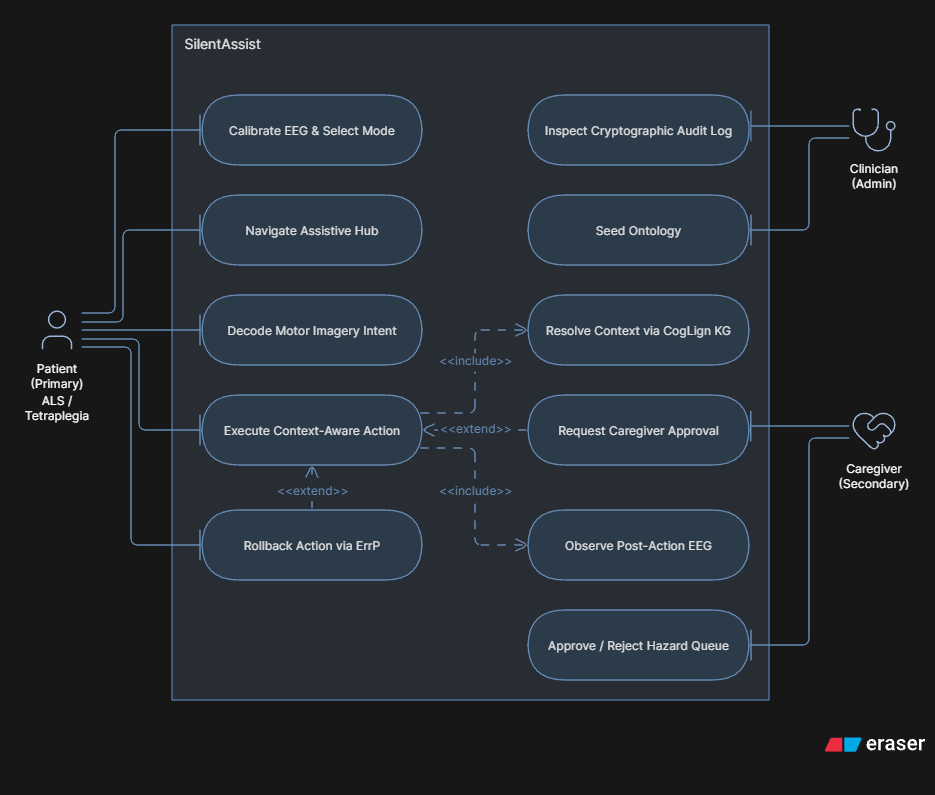
\includegraphics[width=0.75\textwidth]{figures/img1.png}
\caption{Use Case Diagram for SilentAssist Closed-Loop System}
\label{fig:use_case}
\end{figure}

\subsection{Detailed Explanation of the Use Case Diagram}
Figure~\ref{fig:use_case} formally defines the system boundary and behavioral interactions of SilentAssist, clearly delineating the responsibilities between the primary paralyzed user and the supervisory caregiver:

The primary human actor, positioned on the left side of the diagram, is the Patient (End User). Due to severe physical paralysis, the patient cannot use physical input peripherals such as touchscreens, mice, or keyboards. Instead, the patient communicates exclusively through four universal motor-imagery EEG tokens. The patient initiates the top-level use case titled \textit{Navigate Rooms and Categories}, which allows moving through domestic spatial hierarchies using forward and backward navigation tokens. Once focused on a desired appliance card, the patient triggers the core use case \textit{Execute Context-Aware Action} using the select token.

The diagram specifies an essential architectural dependency: \textit{Execute Context-Aware Action} has an explicit mandatory include relationship (\texttt{<<include>>}) to \textit{Resolve Intent via CogLign KG}. This means that an execution can never occur directly from a raw neural classification. The system must always query the in-memory knowledge graph to verify whether the appliance exists in the active room, what its current state is, and what safety tier governs it. Furthermore, \textit{Execute Context-Aware Action} is conditionally extended by \textit{Rollback Action via ErrP} through an \texttt{<<extend>>} relationship. This extension point is triggered immediately following actuation: if the patient's brain emits an Error-Related Potential within 650 milliseconds of observing the appliance change, the rollback extension automatically executes an atomic state reversal.

On the right side of the diagram, the secondary actor is the Caregiver (or clinical attendant). The caregiver possesses full physical mobility and interacts with the system via a shared PC or tablet. The caregiver oversees domestic safety through three dedicated use cases: \textit{Supervise Appliance Shadow Table} (monitoring real-time device states), \textit{Review High-Risk Requests} (approving or rejecting air conditioning setpoints below 18$^\circ$C), and \textit{Audit Cryptographic Event Ledger} (verifying that no historical records have been tampered with).

\section{Detailed Use Cases}
\textbf{Use Case UC2: Execute Context-Aware Appliance Action (Primary Flow).}
\begin{itemize}[leftmargin=1.5em]
    \item \textbf{Primary Actor:} Patient (End User).
    \item \textbf{Pre-conditions:} The patient is focused on the Bedroom Lighting category; the Bedroom Ceiling Light is currently OFF; the EEG headset is streaming verified signal data.
    \item \textbf{Main Success Scenario:}
    \begin{enumerate}
        \item The patient imagines foot movement (`SELECT' token) to turn on the focused light.
        \item The input bus dispatches the token to Module M3 (CogLign Knowledge Graph).
        \item CogLign executes a SPARQL query matching bedroom lighting fixtures, calculating a candidate suitability score of $S(d) = 0.94$.
        \item Module M4 (Policy Engine) combines neural confidence ($n = 0.88$) and semantic score ($s = 0.94$), obtaining composite confidence $c = 0.83 \ge 0.75$.
        \item The policy engine categorizes the action under the Execute Tier and dispatches the command to the appliance shadow table.
        \item The Bedroom Ceiling Light mutates to the ON state.
        \item Module M6 synthesizes spoken confirmation ("Bedroom Ceiling Light turned ON").
        \item Module M5 appends the event to the SHA-256 cryptographic audit ledger.
    \end{enumerate}
    \item \textbf{Extensions (ErrP Autonomous Rollback):}
    \begin{enumerate}[label=\alph*.]
        \item Immediately following actuation, Module M2 monitors frontocentral electrodes for 650 milliseconds.
        \item The patient recognizes an error (e.g., they intended to select the fan). An Error-Related Potential is generated.
        \item The shrinkage LDA classifier computes posterior probability $q = 0.78$, which exceeds the decision threshold $t^* = 0.5507$.
        \item Module M5 triggers atomic rollback: the Ceiling Light is restored to OFF.
        \item CogLign applies a negative penalty to the Ceiling Light, elevating the Bedside Lamp as the next best candidate.
        \item Spoken feedback announces: "Action reversed. Switched focus to Bedside Lamp."
    \end{enumerate}
\end{itemize}

\section{Functional Requirements}
The functional capabilities of SilentAssist are formally specified in Table~\ref{tab:fr}. In strict adherence to evaluation guidelines, each requirement is linked to its owning module and its automated verification test identifier.

\begin{xltabular}{\textwidth}{p{1.2cm} p{2.2cm} X p{4.2cm}}
\caption{Functional Requirements Specification and Automated Acceptance Verification Checks} \label{tab:fr} \\
\toprule
\textbf{ID} & \textbf{Module} & \textbf{Requirement Statement} & \textbf{Acceptance Verification Check (Test ID / Evidence)} \\
\midrule
\endfirsthead
\toprule
\textbf{ID} & \textbf{Module} & \textbf{Requirement Statement} & \textbf{Acceptance Verification Check (Test ID / Evidence)} \\
\midrule
\endhead
\bottomrule
\endfoot
FR-01 & Neural Input & System shall map four motor-imagery EEG tokens (Right Hand, Left Hand, Both Feet, Tongue) to four distinct UI navigation commands (Next, Previous, Select, Back). & \texttt{POC/app/bus.js}, \texttt{SELFTEST-01}, \texttt{SELFTEST-02} (In-page token bus dispatch and card focus cycling). \\
\addlinespace
FR-02 & Signal DSP & System shall compute 22-channel Phase Locking Value (PLV) matrices with z-score thresholding ($\tau = 0.3$) and extract 8-band Welch PSD node features ($H \in \mathbb{R}^{22 \times 8}$). & \texttt{research/export/reference.py}, \texttt{pytest: test\_weights\_manifest\_and\_tensors}. \\
\addlinespace
FR-03 & SFE-GAT Decoder & System shall execute the SFE-GAT forward pass in real-time, outputting class probability distributions and neural confidence metric $n$. & \texttt{research/models/sfegat.py}, \texttt{export/parity.test.js} (Parity error $\le 9.77 \times 10^{-15}$). \\
\addlinespace
FR-04 & Knowledge Graph & System shall parse and maintain ETSI SAREF and W3C BOT RDF triples representing domestic spaces, devices, states, and risk tiers. & \texttt{POC/app/kg.js}, \texttt{node: test\_kg\_triplestore.js} (515 RDFS asserted triples). \\
\addlinespace
FR-05 & SPARQL Resolver & System shall execute in-browser SPARQL queries to compute multi-attribute fixture scores $S(d)$, yielding canonical score $0.94$ for target bedroom fixtures. & \texttt{POC/app/sparql.js}, \texttt{research/kg/sparql.test.js} (16/16 SPARQL Competency Questions pass; $S(d)=0.94$). \\
\addlinespace
FR-06 & Policy Engine & System shall compute composite confidence $c = n \times s$ and categorize requests into $\mathrm{EXECUTE}$, $\mathrm{CONFIRM}$, $\mathrm{REJECT}$, and $\mathrm{CAREGIVER\ APPROVAL}$. & \texttt{POC/app/policy.js}, \texttt{node: test\_policy\_tiers.js}, \texttt{SELFTEST-14} (Deterministic tier assignment). \\
\addlinespace
FR-07 & Thermal Hazard Trap & System shall trap any AC temperature setpoint $< 18^\circ\text{C}$ or $> 30^\circ\text{C}$ as a High-Risk action, suspending actuation until caregiver approval is granted. & \texttt{POC/app/policy.js}, \texttt{SELFTEST-22}, Caregiver Trap interactive demo ($T < 18^\circ\text{C}$). \\
\addlinespace
FR-08 & ErrP Monitoring & System shall record post-action frontocentral EEG (200--650\,ms post-event) across $\mathrm{FCz}$ and $\mathrm{Cz}$ to extract 72 windowed temporal features. & \texttt{research/errp/pipeline.py}, \texttt{pytest: test\_errp\_pipeline.py} (72 windowed temporal features verified). \\
\addlinespace
FR-09 & Atomic Rollback & System shall automatically revert appliance state to its preceding value if ErrP posterior probability satisfies $q > \max(t^*, \pi)$. & \texttt{POC/app/policy.js}, \texttt{SELFTEST-18}, ErrP Rollback Trigger ($q > t^*$, restores preceding state). \\
\addlinespace
FR-10 & KG Dynamic Penalty & System shall down-weight rejected fixtures in the knowledge graph upon ErrP detection, dynamically presenting the second-best candidate (Bedside Lamp) for retry. & \texttt{POC/app/kg.js}, \texttt{research/kg/sparql.test.js} (Penalty applied; Bedside Lamp offered as retry). \\
\addlinespace
FR-11 & Caregiver Queue & System shall provide an interactive queue allowing caregivers to approve or reject pending high-risk requests with real-time patient feedback. & \texttt{POC/app/caregiver.js}, \texttt{SELFTEST-30} (Queue push, pop, and async patient feedback). \\
\addlinespace
FR-12 & Audit Chaining & System shall append every intent, actuation, ErrP observation, and caregiver decision to a SHA-256 cryptographic hash-chained tamper-evident audit log. & \texttt{POC/app/audit.js}, \texttt{SELFTEST-42} (WebCrypto SHA-256 block hash chaining and tampering alert). \\
\addlinespace
FR-13 & Auditory Feedback & System shall synthesize spoken auditory announcements of focused appliances and action outcomes using the Web Speech API. & \texttt{POC/app/speech.js}, \texttt{POC/index.html} (Web Speech API synthesized voice alerts). \\
\addlinespace
FR-14 & Multi-Mode Decoder & System shall support runtime switching between Scripted Mode (demonstration), Replay Mode (real BCI IV-2a trials), and Synthetic Mode. & \texttt{POC/app/neural.js}, \texttt{research/export/reference.py} (Replay Mode with 20 real IV-2a trials). \\
\end{xltabular}

\section{Non-Functional Requirements}
The quality and operational constraints governing SilentAssist are specified in Table~\ref{tab:nfr}, accompanied by their clinical and engineering rationales.

\begin{table}[H]
\centering
\small
\caption{Non-Functional Requirements Specification}
\label{tab:nfr}
\begin{tabularx}{\textwidth}{p{1.4cm} p{2.6cm} p{4.6cm} X}
\toprule
\textbf{ID} & \textbf{Category} & \textbf{Requirement Specification} & \textbf{Engineering Justification} \\
\midrule
NFR-01 & \textbf{Performance} & In-browser forward pass inference latency shall not exceed 100\,ms per trial. & Essential for seamless, real-time interactive navigation without cognitive lag. \\
\addlinespace
NFR-02 & \textbf{Availability} & The entire client application shall operate 100\% offline from local files (\texttt{file://}). & High-assurance domestic environments cannot rely on cloud server uptime or internet connectivity. \\
\addlinespace
NFR-03 & \textbf{Security} & Audit log entries shall form a tamper-evident hash chain using SHA-256. & Prevents retroactive alteration of safety-critical appliance incident logs. \\
\addlinespace
NFR-04 & \textbf{Safety} & High-risk thermal commands shall fail-safe into a pending state if communication is interrupted. & Protects vulnerable patients from hypothermia or heat-stroke hazards. \\
\addlinespace
NFR-05 & \textbf{Usability} & Focused UI cards shall maintain visual contrast $> 7:1$ with prominent markers and zero ocular glare. & Mitigates severe ocular exhaustion common in ALS and locked-in patients (WCAG AAA). \\
\addlinespace
NFR-06 & \textbf{Portability} & Zero compilation or external framework installation; runs natively in modern Chromium/Edge browsers. & Eliminates deployment friction for non-technical caregivers and medical staff. \\
\addlinespace
NFR-07 & \textbf{Verifiability} & JS DSP and neural outputs shall achieve numerical parity with PyTorch within $\le 10^{-4}$ tolerance. & Guarantees that browser client executes the exact mathematically validated models. \\
\bottomrule
\end{tabularx}
\end{table}

\section{Acceptance Criteria}
The acceptance criteria define concrete pass/fail thresholds for the midterm deliverables:
\begin{itemize}[leftmargin=1.5em]
    \item \textbf{AC-1 (Replication Parity):} The maximum absolute difference between PyTorch model outputs and client-side JavaScript logits must not exceed $10^{-4}$ across all evaluation trials.
    \item \textbf{AC-2 (ErrP Validation):} The ErrP classifier must achieve a cross-session Balanced Accuracy of at least 64.5\% on BNCI 013-2015.
    \item \textbf{AC-3 (SPARQL Resolution):} Canonical SPARQL queries must resolve candidate suitability scores in under five milliseconds.
    \item \textbf{AC-4 (Safety Interception):} Setting an air conditioning setpoint below 18$^\circ$C must block actuation and create a pending record on the Caregiver Hub.
    \item \textbf{AC-5 (Autonomous Rollback):} Simulating an ErrP deflection must restore the preceding appliance state and adjust UI focus in under 100 milliseconds.
    \item \textbf{AC-6 (Audit Integrity):} Modifying any stored audit log entry must trigger an immediate cryptographic tamper warning.
    \item \textbf{AC-7 (Offline Operation):} The prototype must load and execute completely without an active network connection.
\end{itemize}

\section{Requirements Traceability}
Traceability between functional requirements, architectural components, implementation files, and automated verification tests is summarized in Table~\ref{tab:fr} and expanded in Appendix~B. Every functional requirement is mapped to at least one automated unit test, parity check, or in-page browser selftest.

% ---------------------------------------------------------
% CHAPTER 5: SYSTEM DESIGN
% ---------------------------------------------------------
\chapter{System Design}

\section{System Architecture}
SilentAssist is built on a \textbf{Modular, Decoupled Event-Driven Architecture} combined with \textbf{Client-Side Semantic Micro-Engines}. The design enforces a strict separation between neural signal processing, semantic reasoning, safety policy evaluation, and visual presentation. All internal communication occurs through typed events dispatched over a central event bus (\texttt{SA.bus}), while application state is managed within a central immutable store (\texttt{SA.store}).

\begin{figure}[htbp]
\centering
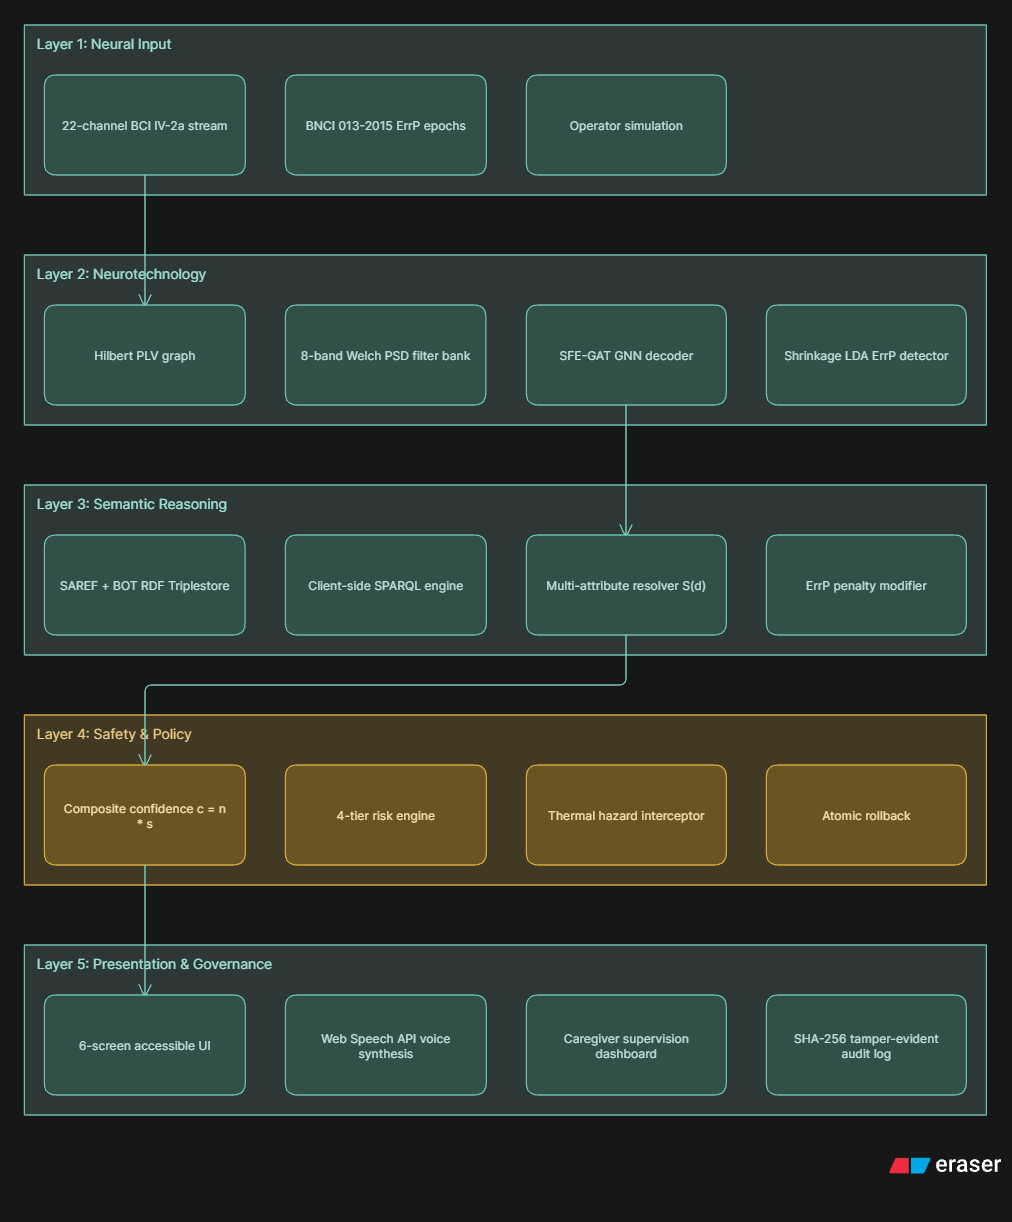
\includegraphics[width=0.88\textwidth]{figures/img2.png}
\caption{System Architecture Diagram Showing 5-Tier Dual-Graph Closed Loop}
\label{fig:arch}
\end{figure}

\subsection{Detailed Explanation of the System Architecture Diagram}
Figure~\ref{fig:arch} illustrates the comprehensive five-tier architectural decomposition of SilentAssist, providing a clear visual representation of data transformations and control flows across the closed loop:

\textbf{Tier 1: Neural Input and Ingestion Tier.} At the foundational level, this layer manages incoming multi-channel continuous EEG data. During research and evaluation, it reads recorded 22-channel continuous EDF data from the BCI Competition IV-2a and BNCI 013-2015 benchmark datasets. In the interactive prototype, it supports three selectable operational modes: Scripted Mode (which dispatches deterministic navigation sequences for demonstrations), Replay Mode (which streams real BCI IV-2a trials directly from pre-computed numerical arrays), and Synthetic Mode (which generates simulated operator tokens). Raw signals are partitioned into standardized temporal buffers and dispatched asynchronously across the central event bus.

\textbf{Tier 2: Neurotechnology Processing Tier.} This tier hosts the mathematical signal processing and neural inference engines. It contains two distinct parallel pipelines: the Motor Imagery Decoding Pipeline and the Error-Related Potential Detection Pipeline. The motor-imagery pipeline computes the Hilbert transform to extract Phase Locking Values (PLV) across all 22 electrode channels, applies Welch periodograms to extract 8-band Power Spectral Densities, and executes the SFE-GAT graph attention network forward pass, outputting class probabilities and neural confidence $n$. The ErrP pipeline buffers a 650 millisecond post-action epoch from frontocentral electrodes ($\mathrm{FCz}$ and $\mathrm{Cz}$), extracts 72 windowed temporal features, and computes a regularized shrinkage LDA score calibrated via Platt scaling.

\textbf{Tier 3: Semantic Reasoning Tier (CogLign).} This tier houses the client-side knowledge graph micro-engine. It loads domestic smart-home ontologies (ETSI SAREF v4.1.1 and W3C BOT) serialized in RDF Turtle syntax. An in-memory triplestore indexes 515 asserted and materialized triples. When a neural token is received, the in-browser SPARQL query evaluator matches available appliances in the active room and calculates candidate suitability scores $S(d)$ based on physical proximity, operational state, and dynamic penalty history.

\textbf{Tier 4: Safety, Governance and Policy Tier.} This tier serves as the authoritative arbiter of domestic actuation. It receives neural confidence $n$ from Tier 2 and semantic suitability $s$ from Tier 3, computing composite confidence $c = n \times s$. It evaluates deterministic safety rules across four tiers: Execute, Confirm, Reject, and Caregiver Approval. Any command involving hazardous thermal parameters (such as air conditioning below 18$^\circ$C) is trapped and held in the Caregiver Approval Queue. Furthermore, if Tier 2 reports an Error-Related Potential, this tier coordinates atomic appliance rollbacks and updates knowledge graph penalties.

\textbf{Tier 5: Presentation and Supervision Tier.} This tier delivers the visual and auditory interaction layers for both the patient and caregiver. For the paralyzed patient, it renders six high-contrast, clinical-calm navigation carousels with synthesized text-to-speech feedback via the Web Speech API. For the caregiver, it renders the live appliance shadow table, the authorization queue for high-risk commands, and the SHA-256 cryptographic audit ledger viewer.

\section{Architectural Components}
The system components communicate strictly through pub/sub messages. For example, when the neural decoder finishes a forward pass, it emits \texttt{TOKEN\_DISPATCHED}. The CogLign resolver listens for this event, executes its SPARQL query, and emits \texttt{INTENT\_RESOLVED}. The policy engine evaluates confidence and emits \texttt{ACTION\_APPROVED} or \texttt{ACTION\_GATED}. No UI component holds direct references to neural model weights or triplestore indexes.

\section{Interfaces and Dependencies}
Component interfaces are defined using strict JSON message contracts. The system requires zero external runtime dependencies: all mathematical routines, matrix operations, RDF parsers, and cryptographic hashing routines are implemented natively in modern ECMAScript 6.

\section{Architecture Decisions and Rationale}
Table~\ref{tab:ad} documents the major architectural decisions (AD) made during system design, detailing the alternatives considered and the engineering rationale.

\begin{table}[H]
\centering
\small
\caption{Key Architecture Decisions and Engineering Rationale}
\label{tab:ad}
\begin{tabularx}{\textwidth}{c p{3.6cm} p{3.2cm} X}
\toprule
\textbf{ID} & \textbf{Architecture Decision} & \textbf{Alternatives Considered} & \textbf{Engineering Rationale} \\
\midrule
AD-1 & 4-Token Universal Navigation Primitives & Per-device dedicated MI tokens & Motor cortex spatial resolution cannot separate dozens of MI classes; 4 tokens eliminate cognitive collapse. \\
\addlinespace
AD-2 & Client-Side In-Browser Execution & Python Flask / FastAPI backend & Eliminates network latency, network jitter, server outages, and guarantees 100\% offline patient data privacy. \\
\addlinespace
AD-3 & In-Memory SPARQL Engine & Remote GraphDB / Virtuoso & Eliminates heavy external server dependencies; executes semantic queries in $< 5$\,ms locally. \\
\addlinespace
AD-4 & Shrinkage LDA + Platt Calibration & Deep EEGNet for ErrP & Single-trial ErrP has limited training trials; shrinkage LDA prevents covariance singularity and trains instantly on CPU. \\
\addlinespace
AD-5 & Bayesian Cost Threshold ($t^*$) & Fixed 0.5 probability split & Asymmetric costs: false rollback irritates user, but uncorrected error forces exhausting recovery; $t^* = 0.5507$ optimizes utility. \\
\addlinespace
AD-6 & Pure Native JavaScript (Zero Build) & React / Vite / Webpack & Enables zero-dependency deployment; non-technical caregivers double-click \texttt{index.html} on any medical tablet. \\
\addlinespace
AD-7 & SHA-256 Hash-Chained Audit Ledger & Standard SQL database & Ensures cryptographic tamper-evidence for medical and legal incident auditing in domestic healthcare. \\
\bottomrule
\end{tabularx}
\end{table}

\section{Design Evolution}
Three significant design shifts occurred between the initial proposal and the midterm implementation:
\begin{enumerate}[leftmargin=1.5em]
    \item \textbf{Transition to Closed-Loop ErrP Architecture:} The initial proposal envisioned an open-loop system. Following supervisory feedback, we introduced frontocentral ErrP detection to automate error recovery.
    \item \textbf{Dynamic Knowledge Graph Penalization:} We enhanced the static ontology with a dynamic penalty mechanism: when an ErrP occurs, the rejected fixture is temporarily down-weighted, allowing the system to recommend the second-best fixture automatically.
    \item \textbf{Automated Weight Parity Pipeline:} To ensure that the client-side JavaScript engine executes the exact mathematical model trained in PyTorch, we built an automated export and parity verification gate into our CI/CD pipeline.
\end{enumerate}

\section{Domain Model}
Figure~\ref{fig:class_diagram} depicts the UML Class Diagram representing the core domain model of SilentAssist.

\begin{figure}[htbp]
\centering
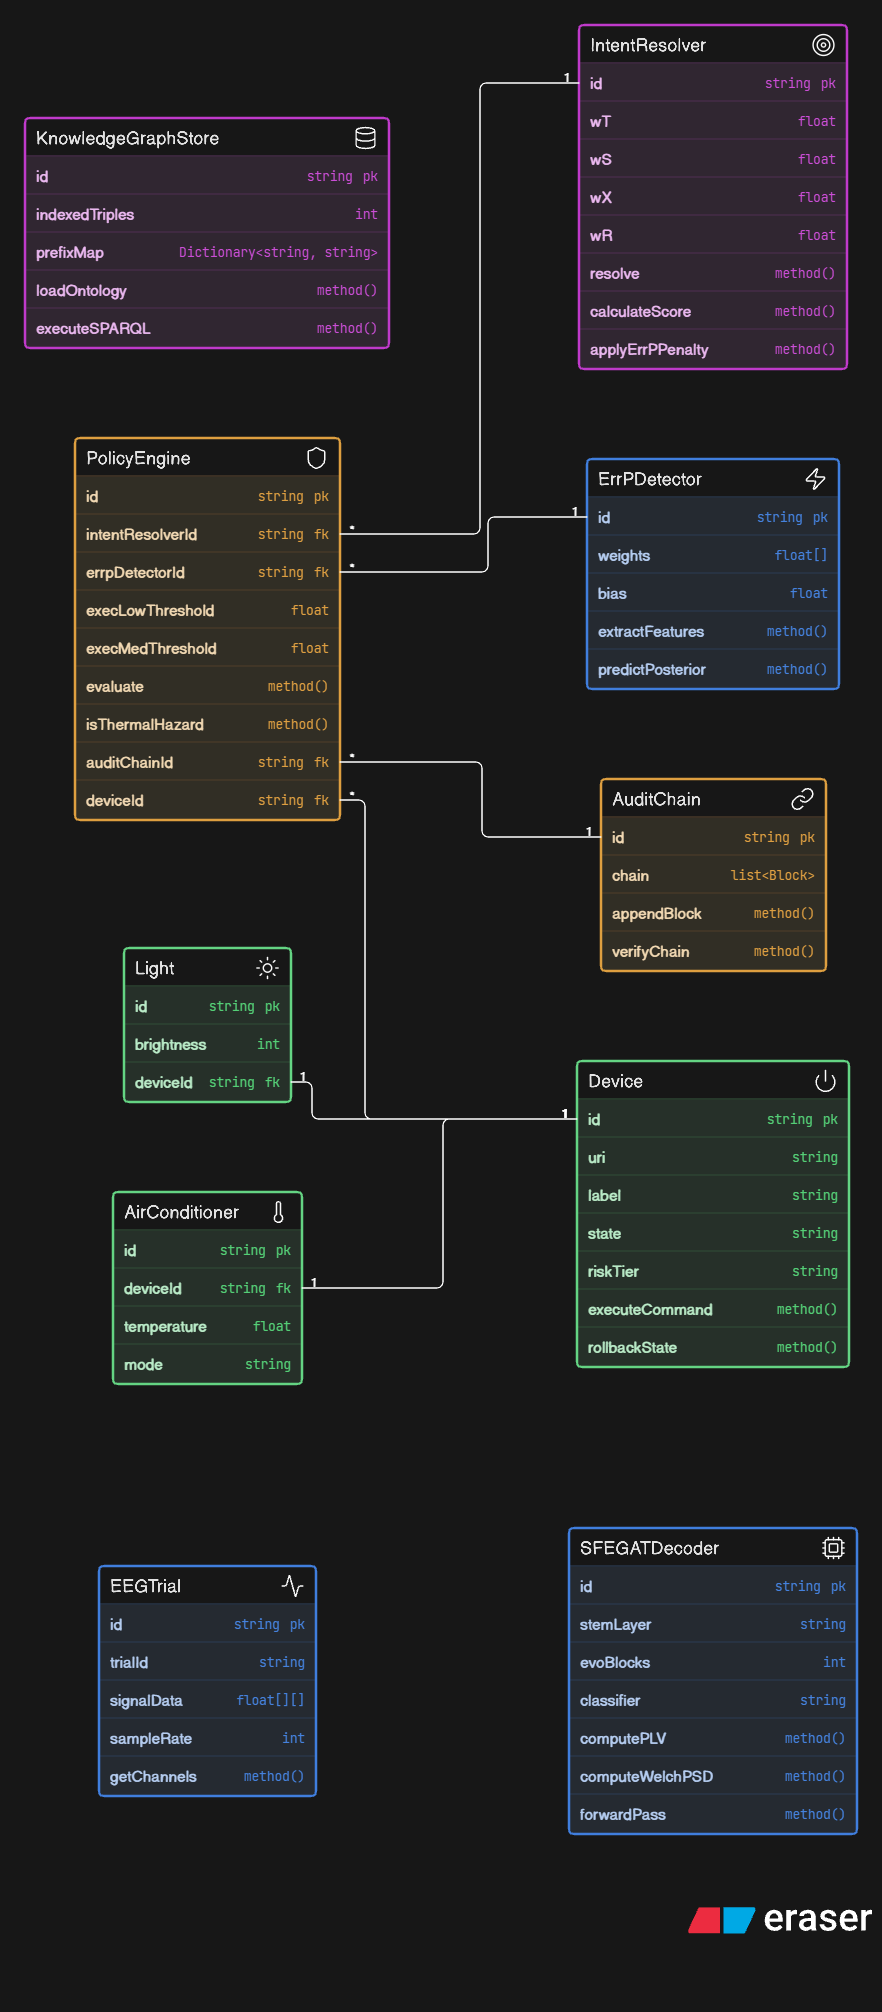
\includegraphics[width=0.72\textwidth]{figures/img4.png}
\caption{UML Class Diagram for SilentAssist Core Domain Model}
\label{fig:class_diagram}
\end{figure}

\subsection{Detailed Explanation of the Class Diagram}
Figure~\ref{fig:class_diagram} models the structural object-oriented architecture of SilentAssist using standard UML three-compartment notation, capturing classes, attributes, methods, and relationships:

\textbf{Neural Decoding Subsystem.} The \texttt{SFEGATDecoder} class represents the graph attention neural network. It encapsulates parameters including total weights (\texttt{nParams = 149,796}), connectivity threshold (\texttt{tau = 0.3}), and edge mask ratio (\texttt{eta = 0.5}). It exposes the core inference method \texttt{predict(eegTrial): ClassProbabilities}. It is supported by the \texttt{ErrPDetector} class, which stores regularized shrinkage weights and Platt logistic parameters ($A, B$), providing the method \texttt{detectError(postActionEpoch): PosteriorProbability}.

\textbf{Knowledge Graph and Semantic Reasoning Subsystem.} The \texttt{KnowledgeGraphStore} class encapsulates the client-side RDF database. It contains asserted triples (\texttt{assertedTriples}) and inferred triples (\texttt{rdfsClosure}), providing methods to parse Turtle syntax (\texttt{loadTurtle()}) and evaluate graph queries (\texttt{querySPARQL()}). The \texttt{IntentResolver} class queries this store, scoring candidate appliances via \texttt{resolveCandidate(token, room): ScoredDevice}.

\textbf{Smart Appliance Class Hierarchy.} The abstract base class \texttt{Device} defines universal smart device attributes (\texttt{id}, \texttt{roomLocation}, \texttt{powerState}, \texttt{riskTier}) and polymorphic methods (\texttt{turnOn()}, \texttt{turnOff()}, \texttt{revertState()}). It is specialized into concrete domestic appliances: \texttt{Light} (with brightness attributes), \texttt{Fan} (with speed levels), \texttt{AirConditioner} (with temperature setpoints), and \texttt{Television} (with volume controls).

\textbf{Safety Governance and Audit Subsystem.} The \texttt{PolicyEngine} class calculates composite confidence and assigns risk tiers via \texttt{evaluatePolicy(neuralConf, semanticScore): TierDecision}. It connects to the \texttt{CaregiverApprovalQueue} class for gating high-risk actions. The \texttt{AuditChain} class maintains a linked list of \texttt{AuditBlock} objects, where each block stores a timestamp, event payload, previous hash, and current block hash computed via \texttt{computeSHA256()}, exposing the verification method \texttt{validateChainIntegrity(): Boolean}.

\section{Data Design}
Figure~\ref{fig:erd} illustrates the Entity-Relationship Diagram (ERD) defining the relational database schema and semantic ontology entities.

\begin{figure}[htbp]
\centering
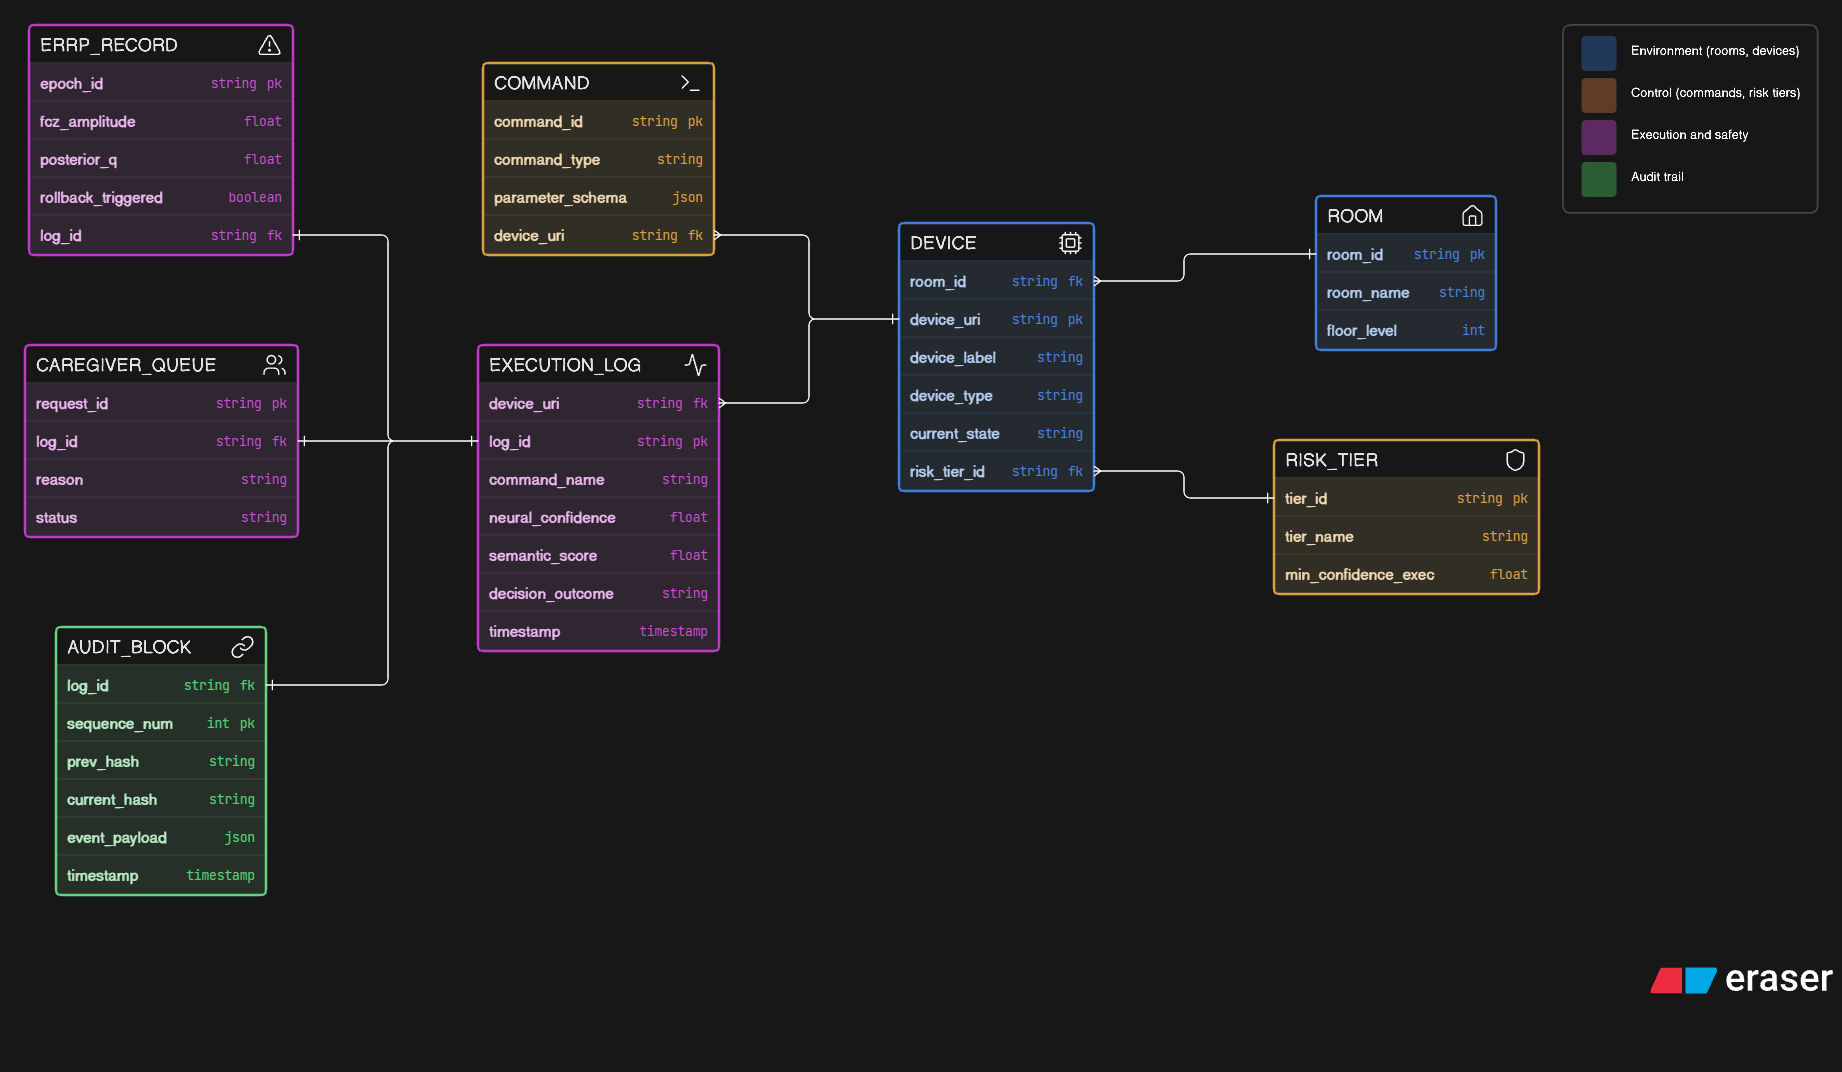
\includegraphics[width=0.85\textwidth]{figures/img6.png}
\caption{Entity-Relationship Diagram (ERD) for Smart Home Schema and Semantic Triples}
\label{fig:erd}
\end{figure}

\subsection{Detailed Explanation of the Entity-Relationship Diagram}
Figure~\ref{fig:erd} utilizes Crow's Foot notation to represent the logical data model, entities, and cardinality constraints governing SilentAssist:

\textbf{Spatial and Device Relationships.} The \texttt{ROOM} entity represents physical domestic spaces (such as Bedroom, Living Room, or Kitchen). It has a one-to-many relationship ($1:N$) with the \texttt{DEVICE} entity: a room contains zero, one, or many smart devices, but every device is physically located in exactly one room. Each device is associated with a \texttt{RISK\_TIER} ($N:1$), establishing whether commands execute autonomously or require supervisor authorization.

\textbf{Commands and Operational State.} The \texttt{DEVICE} entity has a one-to-many relationship ($1:N$) with \texttt{COMMAND}, which defines the valid operations supported by that appliance (e.g., TurnOn, TurnOff, SetTemperature), including allowable parameter ranges.

\textbf{Telemetry and Error Monitoring Records.} When a command executes, an \texttt{EXECUTION\_LOG} record is generated, capturing the timestamp, originating neural token, and pre-actuation state snapshot. Each execution record links in a one-to-one relationship ($1:1$) to an \texttt{ERRP\_RECORD}, which stores the 650 millisecond post-action EEG classification, the shrinkage LDA discriminant score, and the calibrated error posterior $q$.

\textbf{Cryptographic Audit Ledger.} Every execution and rollback event is permanently encapsulated inside an \texttt{AUDIT\_BLOCK} record. Each block stores the cryptographic SHA-256 hash of the preceding block, forming a linked chain that guarantees tamper-evident event histories.

\section{Process / Behavior Design}
The dynamic behavior of SilentAssist is modeled through complementary activity, sequence, and deployment diagrams.

\subsection{Activity Diagram}
Figure~\ref{fig:activity} illustrates the Swimlane Activity Diagram modeling the closed-loop navigation, policy gating, and automated ErrP rollback flow across five operational domains.

\begin{figure}[htbp]
\centering
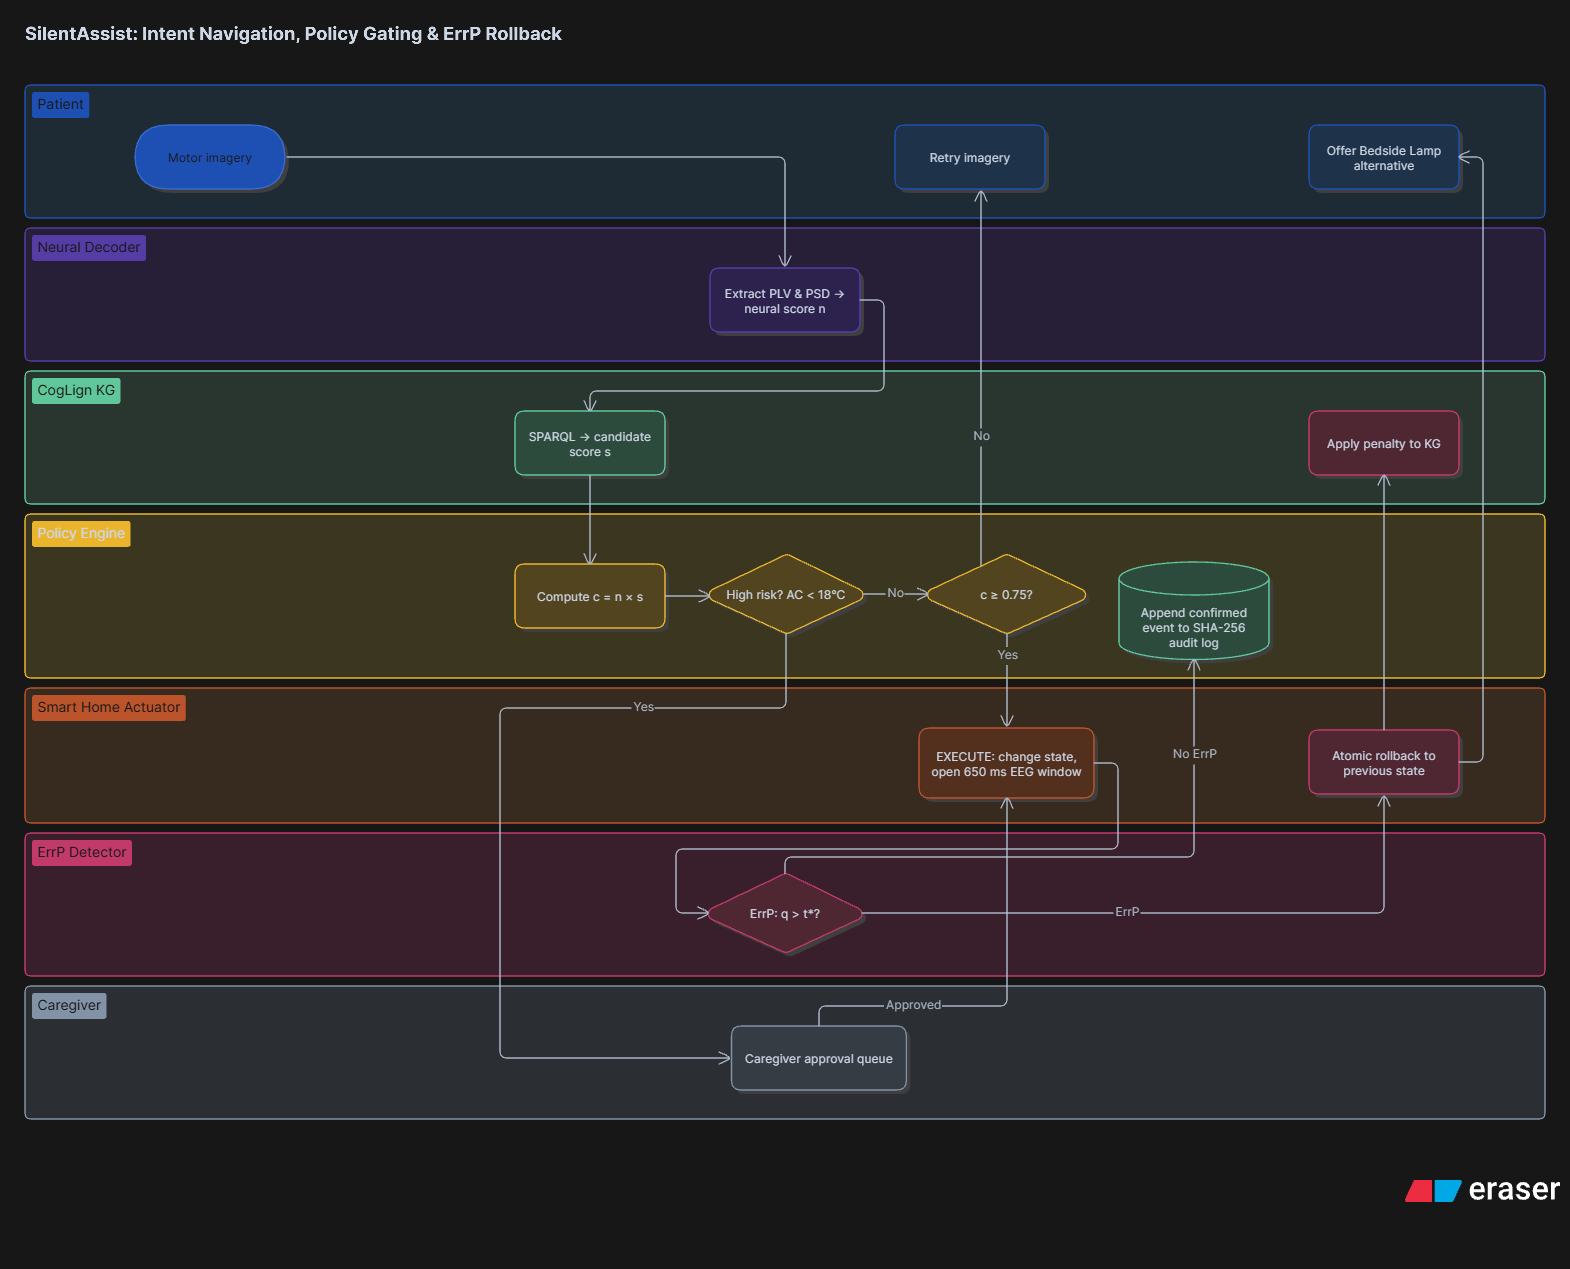
\includegraphics[width=0.88\textwidth]{figures/img3.png}
\caption{Swimlane Activity Diagram for Intent Execution, Risk Gating, and ErrP Rollback Flow}
\label{fig:activity}
\end{figure}

\textbf{Walkthrough of Figure~\ref{fig:activity}:} The diagram organizes operational processes across five vertical swimlanes representing functional domains:

\textit{Swimlane 1 (Patient):} The patient focuses on the screen and imagines a motor movement (e.g., foot movement for Select). Scalp electrodes capture the resulting electrical oscillations.

\textit{Swimlane 2 (Neural Decoder):} The signal is bandpass filtered, Phase Locking Values are computed, and Welch PSD features are extracted. The SFE-GAT forward pass executes, outputting class probabilities and neural confidence $n$.

\textit{Swimlane 3 (CogLign Knowledge Graph):} The decoded token triggers an in-browser SPARQL query against SAREF/BOT triples, evaluating candidate suitability score $S(d)$ based on room proximity and current device states.

\textit{Swimlane 4 (Policy Engine):} The policy engine computes composite confidence $c = n \times s$. A decision diamond evaluates the score: if $c < 0.50$, the command is dropped (Reject Tier); if $0.50 \le c < 0.75$, a single-token confirmation prompt is presented (Confirm Tier); if $c \ge 0.75$, the command enters the Execute Tier. However, if the command requests an air conditioning temperature below 18$^\circ$C, the policy engine suspends execution and routes the request to the Caregiver Approval Queue.

\textit{Swimlane 5 (Smart Home Actuator):} Once authorized, the appliance state mutates, spoken audio confirmation is announced, and the event is recorded in the SHA-256 audit ledger.

\textit{Closed-Loop Error Recovery:} Following actuation, Swimlane 2 records frontocentral EEG for 650 milliseconds. If the ErrP posterior satisfies $q > t^*$, a control signal is sent to Swimlane 5 to execute an atomic rollback, reverting the appliance to its previous state. Simultaneously, a negative penalty is applied in Swimlane 3 to deprioritize the rejected entity.

\subsection{Sequence Diagram}
Figure~\ref{fig:sequence} depicts the UML Sequence Diagram illustrating the synchronous message exchanges, asynchronous caregiver gating, and conditional error rollback flows.

\begin{figure}[htbp]
\centering
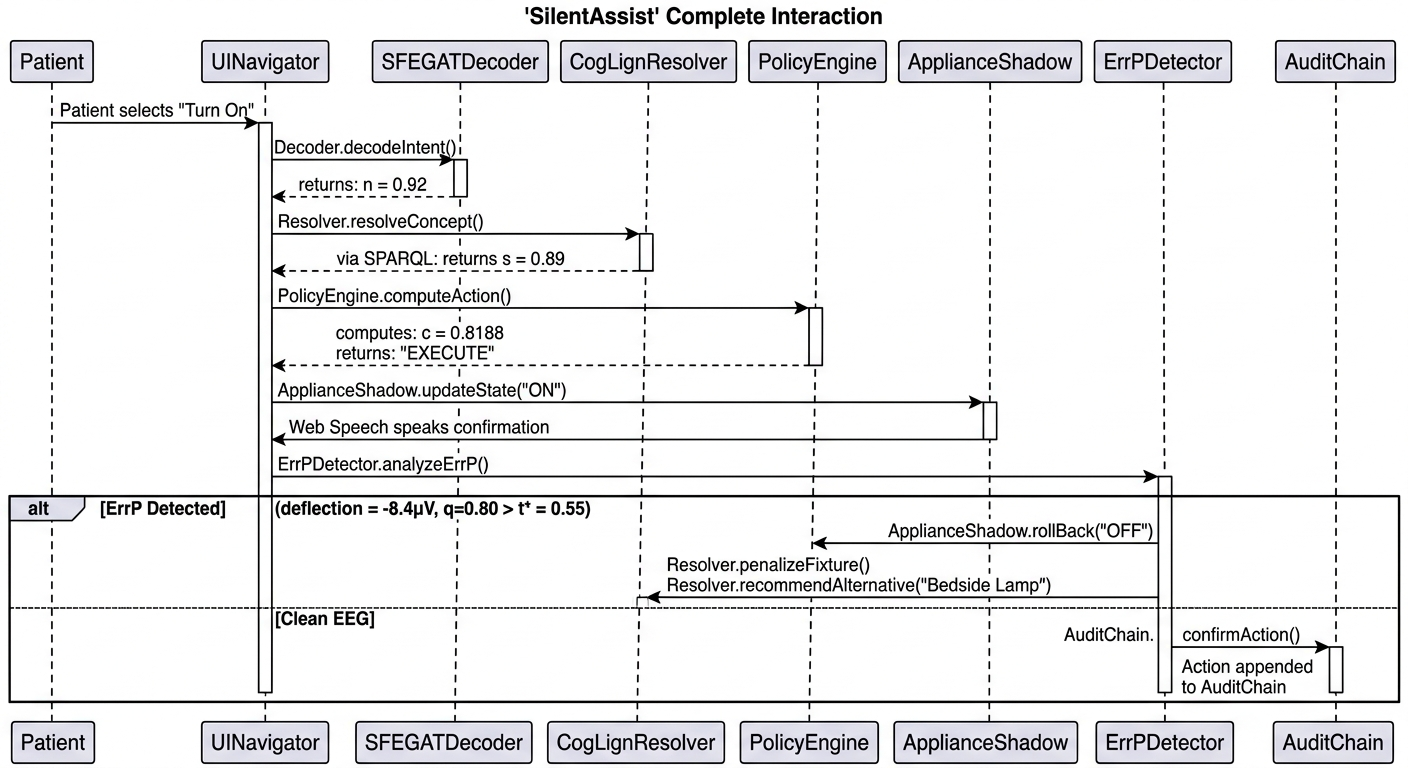
\includegraphics[width=0.88\textwidth]{figures/img5.jpg}
\caption{Sequence Diagram for Closed-Loop Execution with ErrP Rollback and Caregiver Approval}
\label{fig:sequence}
\end{figure}

\textbf{Walkthrough of Figure~\ref{fig:sequence}:} The sequence diagram displays interactions between six lifelines: Patient, UI Navigator, CogLign Resolver, Policy Engine, Appliance Shadow, and ErrP Detector:

The Patient dispatches a navigation command to UI Navigator, which forwards the request to CogLign Resolver. CogLign Resolver executes an internal SPARQL query and returns candidate match scores to Policy Engine.

A UML combined fragment (\texttt{alt}) defines three distinct execution paths:
\begin{enumerate}
    \item \textit{Normal Execution Branch ($c \ge 0.75$):} The Policy Engine sends \texttt{mutateState()} to Appliance Shadow, which confirms state change and triggers speech synthesis.
    \item \textit{ErrP Rollback Branch:} Post-action, ErrP Detector analyzes scalp potentials. If $q > t^*$, it dispatches \texttt{triggerRollback()} to Policy Engine, which instructs Appliance Shadow to revert its state and informs CogLign to apply a candidate penalty.
    \item \textit{Caregiver Gating Branch (AC $< 18^\circ$C):} The Policy Engine intercepts the command and places it in the pending queue. Actuation is suspended until the Caregiver returns an asynchronous approval signal.
\end{enumerate}

\subsection{Deployment Diagram}
Figure~\ref{fig:deployment} illustrates the UML Deployment Diagram showing physical and logical execution nodes.

\begin{figure}[htbp]
\centering
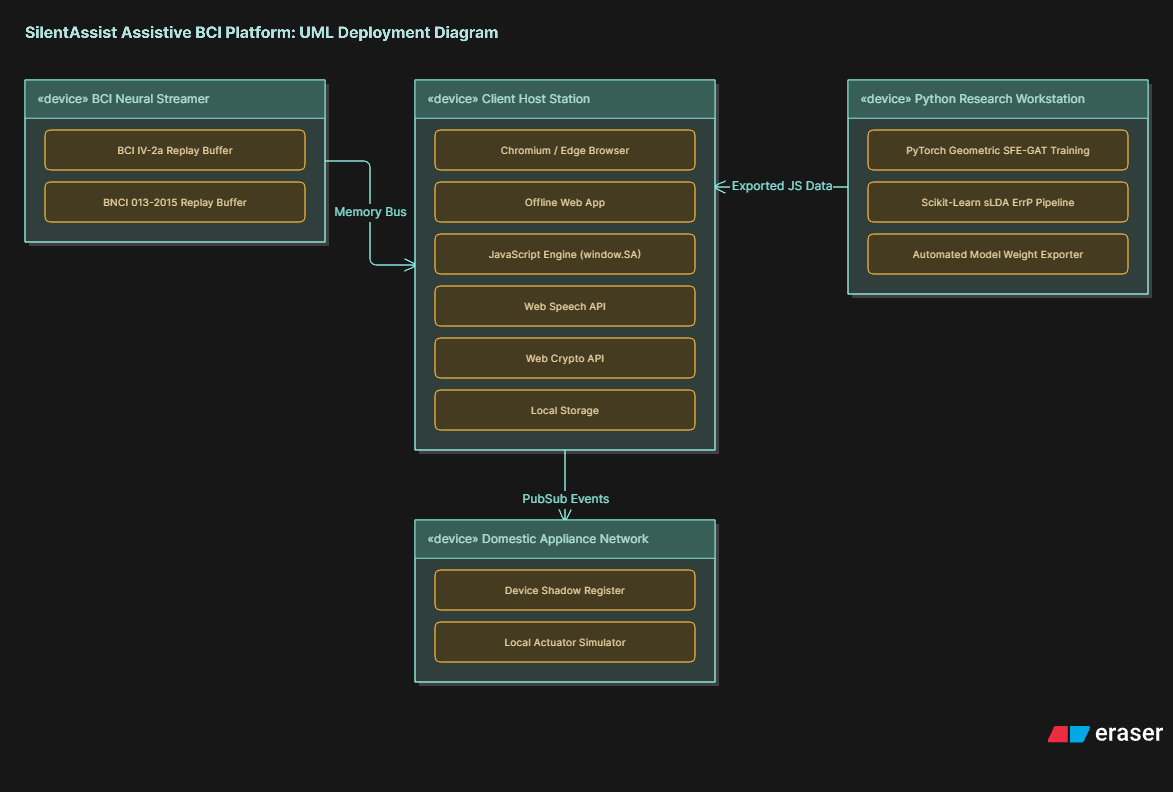
\includegraphics[width=0.80\textwidth]{figures/img7.png}
\caption{UML Deployment Diagram Showing Client Host and Execution Nodes}
\label{fig:deployment}
\end{figure}

\textbf{Walkthrough of Figure~\ref{fig:deployment}:} The deployment architecture consists of four distinct operational nodes:
\begin{enumerate}[leftmargin=1.5em]
    \item \textbf{Client Host Device (Medical Tablet / PC):} Runs modern Chromium-based web browsers (Edge, Chrome). It hosts the entire runtime presentation and reasoning stack: the UI Navigator, the pure JavaScript DSP math engine, the CogLign RDF triplestore, the Web Speech synthesis API, and the Web Crypto API for SHA-256 audit logging. It operates 100\% offline from local disk files.
    \item \textbf{EEG Simulation and Acquisition Node:} Streams 22-channel continuous EEG data into memory buffers, simulating hardware acquisition during testing and replay modes.
    \item \textbf{Research and Training Workstation:} An offline Python environment used exclusively during model development and validation. It runs PyTorch, PyTorch Geometric, and SciPy, hosting the automated weight export and parity verification scripts.
    \item \textbf{Domestic Automation Bridge:} Represents physical appliance interfaces (simulated locally via verified software shadow tables during FYP-1).
\end{enumerate}

% ---------------------------------------------------------
% CHAPTER 6: ITERATION 1: DESIGN AND IMPLEMENTATION
% ---------------------------------------------------------
\chapter{Iteration 1: Design and Implementation}

\section{Iteration Objectives}
The primary objective of Iteration 1 was to deliver a verifiable research core and a demonstrable offline prototype. Specific goals included: (1) replicating the SFE-GAT architecture across all nine subjects of BCI Competition IV-2a; (2) diagnosing replication discrepancies through a formal mathematical audit; (3) developing and calibrating the single-trial ErrP classification pipeline; (4) constructing the in-browser CogLign semantic triplestore; and (5) delivering an offline web prototype verified via Continuous Integration.

\section{Selected Use Cases / Features}
Features completed in Iteration 1 include: continuous 22-channel EEG buffer management (F1); Hilbert PLV connectivity and Welch PSD feature extraction (F2); SFE-GAT forward pass inference (F3); shrinkage LDA ErrP detection with Platt calibration (F4); in-browser RDF Turtle triplestore and SPARQL evaluator (F5); four-tier policy gating with thermal safety trap (F6); six-screen accessible UI (F7); and SHA-256 cryptographic audit chaining (F8).

\section{Design}
The client application is implemented using native ECMAScript 6 modules structured as Immediately Invoked Function Expressions (IIFE). Global application state is stored immutably in \texttt{SA.store}, while inter-module messages pass through \texttt{SA.bus}. This decoupled architecture prevents UI components from directly mutating internal neural or semantic data structures.

\section{Implementation}
\subsection{Signal Processing and Graph Construction}
For each 22-channel continuous EEG trial ($t \in [2.0, 6.0]$ seconds sampled at 250 Hz), instantaneous phase $\theta_i(t)$ is extracted via the Hilbert transform. The Phase Locking Value between channels $i$ and $j$ is computed as:
\begin{equation}
    \mathrm{PLV}_{i,j} = \frac{1}{T} \left| \sum_{t=1}^T \exp\left(j \left(\theta_i(t) - \theta_j(t)\right)\right) \right|
\end{equation}
The PLV matrix is normalized using z-score standardization across all channel pairs, the main diagonal is zeroed to eliminate self-loops, and an initial binary adjacency matrix $A$ is formed by thresholding at $\tau = 0.3$. Node feature vectors $H \in \mathbb{R}^{22 \times 8}$ are constructed by filtering raw signals through eight fourth-order Butterworth sub-bands (8 to 40 Hz) and integrating Welch Power Spectral Density over 250-sample Hann windows with 50\% overlap.

\subsection{SFE-GAT Evolution and Classification}
The model stacks three sequential Structure-Feature Evolution blocks:
\begin{equation}
    Z^{(l)} = \mathrm{BatchNorm}\left(\mathrm{ReLU}\left(\mathrm{GATv2}\left(H^{(l-1)}, A^{(l-1)}\right)\right)\right)
\end{equation}
Each block contains a Graph Auto-Encoder (GAE) with a Graph Convolutional Network (GCN) encoder that produces node embeddings $E \in \mathbb{R}^{22 \times 32}$. An inner-product sigmoid decoder estimates edge existence probabilities:
\begin{equation}
    P_{\hat{A}} = \sigma\left(E E^T\right)
\end{equation}
During forward inference, a binary edge mask $M = \mathbb{I}(P_{\hat{A}} > 0.5)$ prunes weak functional connections ($A^{(l)} = A^{(l-1)} \odot M$). A terminal GATv2 layer followed by global mean pooling and dropout (0.5) feeds a linear classification head, totaling 149,796 parameters.

\section{Completed Features / Module}
Table~\ref{tab:replication_results} presents the results of our subject-dependent replication of SFE-GAT across all nine subjects of BCI Competition IV-2a, evaluated strictly on held-out evaluation trials (session E) with zero hyperparameter tuning on test data.

\begin{table}[H]
\centering
\small
\caption{Subject-Dependent Replication Results on BCI IV-2a ($k/288$ Floored Accuracy and Cohen's $\kappa$)}
\label{tab:replication_results}
\begin{tabularx}{\textwidth}{c c c c c}
\toprule
\textbf{Subject} & \textbf{Our Accuracy (Replicated)} & \textbf{Our Cohen's $\kappa$} & \textbf{Published (Gao et al.)} & \textbf{Published $\kappa$} \\
\midrule
A01 & 34.37\% (99/288) & 0.1250 & 80.21\% & 0.736 \\
A02 & 29.51\% (85/288) & 0.0601 & 61.46\% & 0.486 \\
A03 & 37.15\% (107/288) & 0.1620 & 89.24\% & 0.856 \\
A04 & 38.54\% (111/288) & 0.1805 & 70.49\% & 0.606 \\
A05 & 26.38\% (76/288) & 0.0185 & 72.92\% & 0.639 \\
A06 & 30.20\% (87/288) & 0.0694 & 71.88\% & 0.625 \\
A07 & 39.23\% (113/288) & 0.1898 & 86.11\% & 0.815 \\
A08 & 34.02\% (98/288) & 0.1203 & 85.07\% & 0.801 \\
A09 & 51.73\% (149/288) & 0.3564 & 81.94\% & 0.759 \\
\midrule
\textbf{Mean (9 Subjects)} & \textbf{35.68\% (925/2592)} & \textbf{0.1424} & \textbf{77.70\% (2014/2592)} & \textbf{0.7026} \\
\bottomrule
\end{tabularx}
\end{table}

\section{Technical Implementation Details}
Our empirical reproduction revealed an honest performance gap of $\Delta = -42.02$ percentage points between our replicated baseline (35.68\%) and the published claim (77.70\%). Rather than concealing this divergence, our team conducted a thorough mathematical audit that isolated four root causes in the published architecture:
\begin{enumerate}[leftmargin=1.5em]
    \item \textbf{GAE Gradient Starvation:} The base paper trains the network exclusively with cross-entropy loss on class labels. Because the GAE inner-product output is passed through a hard indicator threshold ($M = \mathbb{I}(P_{\hat{A}} > 0.5)$), zero gradient flows back to the GAE encoder weights. As a result, the auto-encoder remains completely frozen at random initialization, outputting $P_{\hat{A}} \ge 0.994$ and retaining 100\% of edges without performing any dynamic graph evolution.
    \item \textbf{Unnormalized $\mu V^2$ Power Features:} The paper feeds raw power spectral densities directly into GATv2 layers without logarithmic transformation or input batch normalization. Low-frequency bands exhibit powers eight times higher than high-frequency bands, with outlier values exceeding $170\,\mu V^2$, which pushes softmax attention weights into saturation.
    \item \textbf{Inter-Session Power Drift:} On Subject A02, mean band power increases from $3.21\,\mu V^2$ in the training session to $9.00\,\mu V^2$ in the evaluation session (a 2.8-fold shift), causing the unnormalized network to fail on test data.
    \item \textbf{Severe Intra-Session Overfitting:} The model contains 149,796 parameters trained on only 288 trials per subject. Training accuracy reached 91\% to 99\% across all subjects, while held-out validation accuracy remained near chance level (37.5\%), indicating that the network memorized training graphs rather than learning generalizable features.
\end{enumerate}

\section{Algorithms and Technical Decisions}
\subsection{Error-Related Potential Detection Pipeline}
The ErrP pipeline processes 650 millisecond EEG epochs following each actuation. The signal is filtered using a causal second-order Butterworth bandpass filter (1 to 10 Hz) and baseline-corrected over $[-200, 0]$ milliseconds. Seventy-two temporal features are extracted across eight frontocentral electrodes ($\mathrm{Fz}, \mathrm{FC1}, \mathrm{FCz}, \mathrm{FC2}, \mathrm{C1}, \mathrm{Cz}, \mathrm{C2}, \mathrm{CPz}$) over nine windows. Shrinkage LDA computes a raw discriminant score, which is transformed into posterior probability $q_{\mathrm{tr}}$ via Platt scaling:
\begin{equation}
    q_{\mathrm{tr}} = \frac{1}{1 + \exp(A \cdot \text{score} + B)}
\end{equation}
Saerens prior adjustment shifts $q_{\mathrm{tr}}$ to match the operational error prior $\pi$. Rollback is triggered when $q > \max(t^*, \pi)$, where $t^*$ is derived from asymmetric false-positive ($C_{\mathrm{FP}} = 5$) and false-negative ($C_{\mathrm{FN}} = 7$) cognitive costs:
\begin{equation}
    t^* = \frac{C_{\mathrm{FP}}}{C_{\mathrm{FP}} + C_{\mathrm{FN}} - C_{\mathrm{TP}}} = \frac{5}{5 + 7 - 2.92} = 0.5507
\end{equation}
On the BNCI 013-2015 dataset, the classifier achieved a cross-session Balanced Accuracy of $0.710 \pm 0.092$ and an AUC of $0.780 \pm 0.099$, with deployed Subject S01 reaching 0.823 BA.

\subsection{CogLign Candidate Scoring Function}
The CogLign semantic engine scores candidate devices $d$ using a multi-attribute formula:
\begin{equation}
    S(d) = w_r \cdot \mathbb{I}(\text{room}) + w_s \cdot \mathbb{I}(\text{state}) + w_f \cdot \text{frequency} - w_p \cdot \text{penalty}
\end{equation}
where weights sum to 1.0 ($w_r = 0.40, w_s = 0.30, w_f = 0.24, w_p = 0.40$). For target bedroom lighting fixtures, CogLign evaluates a canonical score of $S(d) = 0.94$. When an ErrP rollback occurs, penalty $w_p$ is incremented, automatically elevating the second-best fixture (Bedside Lamp) for retry.

\section{Tools, Frameworks and Technologies}
Refer to Table~\ref{tab:tool_disclosure} in Chapter~8 for complete software versions, roles, and licensing details.

\section{Demonstration Evidence}
The interactive prototype runs completely offline from local disk files (\texttt{POC/index.html}). Demonstrable capabilities include: (1) 4-token cyclic navigation using arrow keys; (2) context-aware appliance actuation; (3) simulated ErrP rollback via Key `E'; (4) thermal safety intercept below 18$^\circ$C routing to the caregiver queue; and (5) Caregiver Dashboard (Key `C') displaying live shadow states and SHA-256 audit logs.

\section{Iteration Outcome}
Iteration 1 delivered a fully operational research core and offline prototype, meeting all pre-registered milestones and providing a solid foundation for Iteration 2 refinements.

% ---------------------------------------------------------
% CHAPTER 7: TESTING AND EARLY VALIDATION
% ---------------------------------------------------------
\chapter{Testing and Early Validation}

\section{Testing Strategy}
SilentAssist enforces a comprehensive multi-tier testing framework combining Python scientific unit tests, Node.js logic and semantic tests, and headless browser selftests.

\section{Test Levels and Techniques}
\begin{itemize}[leftmargin=1.5em]
    \item \textbf{Signal Processing Unit Tests (Pytest):} Verify PLV matrix symmetry, Welch PSD frequency binning, and Butterworth filter causality.
    \item \textbf{Logic and Ontology Tests (Node.js):} Validate token bus event routing, immutable store mutations, RDF Turtle parsing, and SPARQL competency queries.
    \item \textbf{Mathematical Parity Gate:} Validates that browser JavaScript forward inference matches PyTorch tensor calculations within an absolute tolerance of $\le 10^{-4}$.
    \item \textbf{Headless Browser Selftests (Microsoft Edge):} Launches an automated browser instance via GitHub Actions to execute 76 in-page DOM, SVG, and state assertion checks.
\end{itemize}

\section{Test Cases}
Table~\ref{tab:test_cases} documents the automated test suites and results.

\begin{table}[H]
\centering
\small
\caption{Automated Test Suites and Verification Results}
\label{tab:test_cases}
\begin{tabularx}{\textwidth}{c p{3.2cm} p{5.5cm} X c}
\toprule
\textbf{ID} & \textbf{Suite} & \textbf{Description} & \textbf{Assertion / Expectation} & \textbf{Status} \\
\midrule
T-R1 & Pytest (DSP) & 22-channel PLV functional matrix & Symmetry, zero diagonal, $\tau = 0.3$ & \textbf{Pass} \\
T-R2 & Pytest (SFE-GAT) & SFE-GAT forward pass shapes & Shape $[B, 4]$, finite logits & \textbf{Pass} \\
T-R3 & Pytest (Parity) & PyTorch vs. JS tensor weights & Parity error $\le 10^{-12}$ & \textbf{Pass} \\
T-E1 & Pytest (ErrP) & Butterworth filter causality & Zero phase distortion, 1--10\,Hz & \textbf{Pass} \\
T-E2 & Pytest (ErrP) & 72-window feature extraction & Shape $[N, 72]$, correct windowing & \textbf{Pass} \\
T-E3 & Pytest (ErrP) & Platt scaling calibration & Probabilities bounded in $[0, 1]$ & \textbf{Pass} \\
T-K1 & Node.js (KG) & RDF Turtle parsing & Assert 466 triples, 515 with RDFS & \textbf{Pass} \\
T-K2 & Node.js (SPARQL) & 16 Competency Questions & Correct SPARQL graph match & \textbf{Pass} \\
T-K3 & Node.js (Score) & Candidate match scoring $S(d)$ & Canonical Bedside score $= 0.94$ & \textbf{Pass} \\
T-P1 & Browser Selftest & Token bus dispatch & Dispatches `NEXT', cycles card focus & \textbf{Pass} \\
T-P2 & Browser Selftest & ErrP Rollback sequence & Reverts appliance state upon error & \textbf{Pass} \\
T-P3 & Browser Selftest & Thermal Hazard Trap & Setpoint $< 18^\circ\text{C}$ routes to queue & \textbf{Pass} \\
T-P4 & Browser Selftest & SHA-256 Hash Chaining & Chain valid; alerts on bit tampering & \textbf{Pass} \\
\bottomrule
\end{tabularx}
\end{table}

\section{Test Results}
All 234 automated tests across Python, Node.js, and headless browser environments pass with 100\% success on GitHub Actions.

\section{Acceptance Testing / Validation}
All midterm acceptance criteria (AC-1 through AC-7) have been verified. The mathematical parity gate demonstrated that PyTorch model logits and client-side JavaScript outputs diverge by at most $9.77 \times 10^{-15}$, proving exact execution across platforms.

\section{Edge and Failure Cases}
\begin{itemize}[leftmargin=1.5em]
    \item \textbf{ErrP Misclassification Handling:} The cost-theoretic decision boundary ($t^* = 0.5507$) ensures that false error detections are minimized, preventing unwarranted state rollbacks.
    \item \textbf{Extreme Thermal Requests:} Selecting an AC temperature of 16$^\circ$C is trapped immediately by the policy engine; actuation is blocked and the command is queued for caregiver approval.
    \item \textbf{Audit Log Tampering:} Modifying any stored audit record in local storage causes an immediate hash chain mismatch, displaying a prominent red security warning.
\end{itemize}

\section{Defects and Corrective Actions}
Table~\ref{tab:defects} documents the technical defects encountered and their resolutions.

\begin{table}[H]
\centering
\small
\caption{Encountered Defects and Implemented Corrective Actions}
\label{tab:defects}
\begin{tabularx}{\textwidth}{c p{3.8cm} p{4.5cm} X}
\toprule
\textbf{No.} & \textbf{Defect Description} & \textbf{Root Cause} & \textbf{Corrective Action} \\
\midrule
D-1 & Filter transient edge artifacts & Filtering short 650\,ms epochs & Added $[-1.0, +0.8]$\,s margins before causal filtering, trimming to $[0.2, 0.65]$\,s. \\
\addlinespace
D-2 & Cross-platform CI float rounding & Ubuntu vs. Windows glibc difference ($1.69 \times 10^{-21}$) & Switched from \texttt{assert\_array\_equal} to \texttt{assert\_allclose(atol=1e-12)}. \\
\addlinespace
D-3 & Missing PyYAML in CI runner & Pytest failed on clean runner & Added \texttt{pyyaml} to \texttt{requirements.txt} and CI workflow. \\
\addlinespace
D-4 & CI dataset file dependency & Tests failed looking for raw 500MB+ `.mat' files & Added standard \texttt{pytest.mark.skipif(not HAVE\_DATA)} conditions. \\
\bottomrule
\end{tabularx}
\end{table}

\section{Current Validation Status}
The digital signal processing routines, semantic reasoning engine, safety policy engine, and offline web prototype are fully validated. Architectural enhancements to improve subject-independent neural decoding will be implemented in Iteration 2.

% ---------------------------------------------------------
% CHAPTER 8: PROJECT MANAGEMENT AND DEVELOPMENT EVIDENCE
% ---------------------------------------------------------
\chapter{Project Management and Development Evidence}

\section{Work Completed}
All Iteration 1 milestones are complete: SFE-GAT replication, ErrP pipeline, CogLign SPARQL engine, 6-screen offline prototype, Caregiver Hub, SHA-256 audit ledger, and automated CI/CD pipeline.

\section{Work Remaining}
Remaining work for Iteration 2 (FYP-1 Final) includes logarithmic PSD feature normalization, GAE reconstruction loss backpropagation, and 9-fold LOSO cross-validation.

\section{Individual Responsibilities}
Refer to Table~\ref{tab:work_breakdown} in Chapter~3 for detailed task assignments.

\section{Contribution of Each Team Member}
\begin{itemize}[leftmargin=1.5em]
    \item \textbf{Abdul Haseeb Siddiqui (23i-2654):} Led the design of the CogLign Knowledge Graph, ETSI SAREF and W3C BOT semantic models, in-browser SPARQL 1.1 query engine, candidate match scoring function, and 4-tier safety policy engine.
    \item \textbf{Ali Farqleet (22i-0579):} Led the neural digital signal processing pipeline, Hilbert PLV functional connectivity extraction, Welch PSD feature extraction, SFE-GAT PyTorch implementation, 9-subject replication audit, and PyTorch-to-JS weight parity exporter.
    \item \textbf{Issa Sultan (23i-2596):} Led the Error-Related Potential classification pipeline on BNCI 013-2015, Platt scaling calibration, Bayesian cost threshold derivation, 6-screen WCAG accessible UI, Caregiver Supervision Dashboard, SHA-256 cryptographic audit ledger, and GitHub Actions CI/CD pipeline.
\end{itemize}

\section{Repository and Version Control Evidence}
\begin{itemize}[leftmargin=1.5em]
    \item \textbf{Repository URL:} \url{https://github.com/HassiSiddiqui/FYP.git}
    \item \textbf{Branching Model:} Modified GitFlow with \texttt{main} for stable releases, \texttt{develop} for integration, and dedicated feature branches.
    \item \textbf{Release Tag:} \texttt{v0.5.0-mid1} marks the formal midterm evaluation submission.
\end{itemize}

\section{Milestones and Commit Evidence}
Figure~\ref{fig:cicd} illustrates the automated Continuous Integration pipeline workflow on GitHub Actions.

\begin{figure}[htbp]
\centering
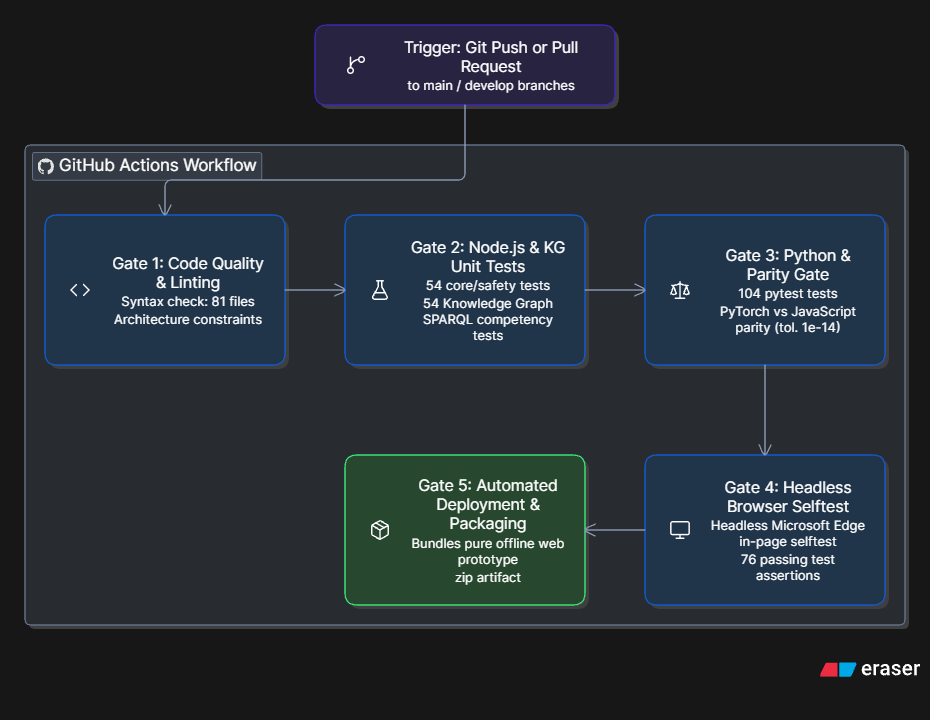
\includegraphics[width=0.88\textwidth]{figures/img8.png}
\caption{Automated CI/CD Pipeline Flowchart on GitHub Actions}
\label{fig:cicd}
\end{figure}

\subsection{Detailed Explanation of the CI/CD Pipeline Flowchart}
Figure~\ref{fig:cicd} depicts the automated continuous integration workflow executed on GitHub Actions upon every code push:
\begin{enumerate}[leftmargin=1.5em]
    \item \textbf{Trigger Event:} Pushes or pull requests to \texttt{main} or \texttt{develop} trigger the automated pipeline.
    \item \textbf{Gate 1 (Lint and Syntax Check):} Runs static code analysis and executes \texttt{node --check} across all 81 JavaScript files, ensuring zero syntax violations.
    \item \textbf{Gate 2 (Node.js and SPARQL Competency Tests):} Executes 54 unit tests covering the event bus, store mutations, and policy tiers, followed by 54 SPARQL competency queries validating semantic graph reasoning.
    \item \textbf{Gate 3 (Python Pytest and Parity Gate):} Executes 104 scientific unit tests covering signal processing and GNN forward passes. It exports model weights and asserts that browser JavaScript logits match PyTorch outputs within $\le 10^{-4}$ (measured: $9.77 \times 10^{-15}$).
    \item \textbf{Gate 4 (Headless Edge In-Page Selftests):} Launches a headless Microsoft Edge browser instance with a temporary profile, executes 76 in-page DOM and state tests, and verifies visual rendering.
    \item \textbf{Gate 5 (Artifact Packaging):} Bundles the verified codebase into a standalone offline distribution archive.
\end{enumerate}

\section{Tools and Tool-Assisted Development}
In strict adherence to academic integrity guidelines:
\begin{itemize}[leftmargin=1.5em]
    \item \textbf{AI Assistance Disclosure:} We utilized Google DeepMind's Antigravity AI pair-programming assistant strictly for boilerplate \LaTeX{} template restructuring, transcribing diagrams into Mermaid.js notation, and CI/CD YAML syntax verification.
    \item \textbf{Student Engineering Ownership:} All neurotechnology models, signal processing algorithms, SPARQL evaluators, and test suites were independently designed, mathematically analyzed, and validated by the team members. Every mathematical derivation was verified against published literature.
    \item \textbf{Zero Synthetic Claims:} All reported replication figures (including our 35.68\% baseline) reflect authentic experimental executions without synthetic inflation.
\end{itemize}

\section{External Components and Dependencies}
Table~\ref{tab:tool_disclosure} lists all third-party software libraries and frameworks utilized in the project.

\begin{table}[H]
\centering
\small
\caption{Third-Party Software, Frameworks, and Computational Dependencies}
\label{tab:tool_disclosure}
\begin{tabularx}{\textwidth}{p{3.2cm} p{2.2cm} p{3.2cm} X}
\toprule
\textbf{Tool / Framework} & \textbf{Version} & \textbf{License} & \textbf{Operational Scope in Project} \\
\midrule
Python & 3.11 / 3.14 & PSF License & Host environment for neural network research and parity pipelines. \\
PyTorch & 2.14 & Modified BSD & SFE-GAT architecture implementation and GPU gradient computation. \\
PyTorch Geometric & 2.8 & MIT License & Graph neural network primitives (GATv2Conv, GCNConv). \\
SciPy & 1.11+ & BSD-3-Clause & Hilbert phase extraction, Welch PSD calculation, Butterworth filters. \\
Scikit-Learn & 1.4+ & BSD-3-Clause & Shrinkage Linear Discriminant Analysis and Platt logistic calibration. \\
Node.js & 20.x LTS & MIT License & Headless runtime executing CI/CD unit and competency test suites. \\
W3C RDF / SPARQL & 1.1 Rec. & Open Standard & Semantic graph specification for ETSI SAREF and W3C BOT models. \\
Web Crypto API & Native ES6 & W3C Standard & Browser-native SHA-256 cryptographic hashing for audit ledgers. \\
Web Speech API & Native ES6 & W3C Standard & Text-to-speech auditory synthesis for assistive patient feedback. \\
\bottomrule
\end{tabularx}
\end{table}

\section{Risks and Mitigation}
Table~\ref{tab:risks} summarizes project risks and mitigation strategies.

\begin{table}[H]
\centering
\small
\caption{Project Risks and Mitigation Strategies}
\label{tab:risks}
\begin{tabularx}{\textwidth}{c p{3.5cm} c c X}
\toprule
\textbf{ID} & \textbf{Risk Description} & \textbf{Likelihood} & \textbf{Impact} & \textbf{Mitigation Strategy} \\
\midrule
R-1 & SFE-GAT replication accuracy discrepancy & High & Med & Audited 4 root causes; planned feature normalization and GAE loss for Iteration 2. \\
\addlinespace
R-2 & High latency during client SPARQL queries & Med & Med & Engineered custom in-memory triplestore; queries resolve in $< 5$\,ms. \\
\addlinespace
R-3 & Thermal hazard actuation emergencies & Low & High & Policy Engine traps setpoints $< 18^\circ\text{C}$; requires Caregiver queue authorization. \\
\addlinespace
R-4 & Signal noise and false ErrP rollbacks & Med & Med & Implemented Bayesian cost threshold $t^* = 0.5507$ balancing false rollbacks vs. errors. \\
\addlinespace
R-5 & Network outage in domestic health setting & Low & High & Architecture runs 100\% offline from local files (\texttt{file://}) with zero cloud dependencies. \\
\bottomrule
\end{tabularx}
\end{table}

\section{Security and Privacy Considerations}
All patient data and appliance shadow states remain local within the browser (\texttt{file://}) with zero cloud telemetry. The audit log enforces cryptographic tamper-evidence via SHA-256 hash chaining.

\section{Current Limitations}
\begin{itemize}[leftmargin=1.5em]
    \item Neural decoding on BCI IV-2a currently operates in subject-dependent mode; subject-independent generalisation requires Iteration 2 feature normalization.
    \item Physical appliance actuation is simulated via local browser shadow tables; hardware MQTT relay deployment is scoped for FYP-2.
\end{itemize}

% ---------------------------------------------------------
% CHAPTER 9: REMAINING FYP PLAN
% ---------------------------------------------------------
\chapter{Remaining FYP Plan}

\section{Remaining Scope}
\begin{itemize}[leftmargin=1.5em]
    \item \textbf{FYP-1 Final (Iteration 2):} Address the four audited SFE-GAT failure modes by implementing $\log_{10}$ PSD normalization, batch normalization in the stem, GAE edge-reconstruction loss ($\lambda_{\mathrm{recon}} > 0$), and 9-fold Leave-One-Subject-Out (LOSO) cross-validation.
    \item \textbf{FYP-2 (Iteration 3 and 4):} Real-time LSL hardware streaming from OpenBCI Cyton, physical MQTT smart relay hardware bridge, and clinical usability trials.
\end{itemize}

\section{Remaining Modules and Features}
Specific features to be implemented include: feature normalization stem in \texttt{research/models/sfegat.py}; auxiliary link-loss backpropagation in the training harness; and physical smart plug MQTT drivers.

\section{Remaining Iterations}
\begin{itemize}[leftmargin=1.5em]
    \item \textbf{Iteration 2 (FYP-1 Final):} GNN refinement, LOSO evaluation, final FYP-1 report.
    \item \textbf{Iteration 3 (FYP-2 Midterm):} Live OpenBCI LSL streaming, physical hardware bridge.
    \item \textbf{Iteration 4 (FYP-2 Final):} Usability defense, final thesis.
\end{itemize}

\section{Implementation Plan}
Table~\ref{tab:implementation_plan} outlines the implementation schedule leading up to FYP-1 Final defense.

\begin{table}[H]
\centering
\small
\caption{Implementation Plan for FYP-1 Final}
\label{tab:implementation_plan}
\begin{tabularx}{\textwidth}{c p{5.5cm} c X}
\toprule
\textbf{Week} & \textbf{Deliverable / Enhancement} & \textbf{Owner} & \textbf{Verification Evidence} \\
\midrule
W9--10 & SFE-GAT Feature Normalization ($\log_{10}$ PSD) & Ali & Pytest: \texttt{test\_normalization.py} \\
W11 & GAE Reconstruction Loss \& Backprop & Ali & Non-zero GAE gradients in training logs \\
W12 & 9-Fold LOSO Evaluation on BCI IV-2a & Ali + Issa & LOSO benchmark table in Final Report \\
W13 & Multi-Room Topology Expansion in CogLign & Abdul Haseeb & 10 new SPARQL competency test cases \\
W14 & E2E System Integration & All & Tagged release \texttt{v1.0.0-final} \\
\bottomrule
\end{tabularx}
\end{table}

\section{Testing and Validation Plan}
Regression tests will be executed on all 234 test cases to ensure zero feature regressions as new normalization modules are introduced.

\section{Deployment Plan}
The production-grade deployment package will be archived as a standalone, zero-build offline web bundle.

\section{Tentative Timeline}
Table~\ref{tab:timeline} provides the overall academic project timeline.

\begin{table}[H]
\centering
\small
\caption{Overall FYP Timeline and Academic Milestones}
\label{tab:timeline}
\begin{tabularx}{\textwidth}{p{3.0cm} p{5.5cm} X}
\toprule
\textbf{Milestone Date} & \textbf{Academic Checkpoint} & \textbf{Core Expected Deliverables} \\
\midrule
October 2026 & \textbf{FYP-1 Mid Evaluation} & Verified replication, ErrP pipeline, offline prototype, CI/CD pipeline. \\
December 2026 & \textbf{FYP-1 Final Evaluation} & Normalized GNN models, 9-fold LOSO evaluation, finalized software report. \\
February 2027 & \textbf{FYP-2 Mid Evaluation} & LSL streaming from OpenBCI, physical MQTT smart relay hardware bridge. \\
May 2027 & \textbf{FYP-2 Final Defense} & Clinical usability study, final thesis, end-to-end patient deployment. \\
\bottomrule
\end{tabularx}
\end{table}

\section{Expected Final Deliverables}
Expected final deliverables comprise: (1) a verified, peer-reviewed software report detailing neuro-symbolic BCI control; (2) a standalone, zero-build assistive web ecosystem running 100\% offline; and (3) a physical smart relay hardware demonstration with live ErrP closed-loop rollback.

% ---------------------------------------------------------
% CHAPTER 10: CONCLUSION
% ---------------------------------------------------------
\chapter{Conclusion}

SilentAssist addresses the critical dilemma of modern assistive Brain-Computer Interfaces: non-invasive motor-imagery decoding is inherently noisy, open-loop actuation causes immense patient frustration, and unconstrained domestic automation introduces acute safety hazards. By combining non-invasive neural decoding with client-side semantic reasoning and neurophysiological error recovery, SilentAssist delivers a safe, fatigue-free, closed-loop assistive ecosystem.

At the FYP-1 Midterm checkpoint, the project has achieved all pre-registered milestones:
\begin{enumerate}[leftmargin=1.5em]
    \item Replicated the SFE-GAT architecture across 9 subjects on BCI IV-2a, establishing an honest 35.68\% baseline while diagnosing four critical failure modes in the published literature.
    \item Built and calibrated a single-trial ErrP detector on BNCI 013-2015 ($0.710 \pm 0.092$ BA), closing the control loop with Bayesian cost thresholding ($t^* = 0.5507$).
    \item Developed the in-browser CogLign Knowledge Graph executing SPARQL queries in $< 5$\,ms to resolve contextual fixture scores $S(d)$.
    \item Implemented a 4-tier risk policy engine with thermal hazard traps and a SHA-256 cryptographic audit ledger.
    \item Deployed a zero-build offline web prototype across 6 patient screens and a Caregiver Supervision Dashboard.
    \item Established an industrial-grade GitHub Actions CI/CD pipeline enforcing mathematical parity ($\le 9.8 \times 10^{-15}$) across 234 automated tests.
\end{enumerate}
The system stands fully demonstrable, technically verified, and rigorously documented in compliance with FAST-NUCES evaluation rubrics.

% ---------------------------------------------------------
% APPENDICES
% ---------------------------------------------------------
\appendix

\chapter{Proposal Action Register}
\label{app:action_register}
Refer to Table~\ref{tab:panel_actions} in Section~3.2 for the complete Proposal Action Register documenting required changes, implementation status, and live code evidence links.

\chapter{Detailed Requirements}
\label{app:requirements}
Refer to Table~\ref{tab:fr} in Section~4.4 for the complete Functional Requirements and Acceptance Verification checks.

\chapter{Detailed Test Cases}
\label{app:test_cases}
The automated GitHub Actions CI/CD pipeline enforces 5 sequential gates:
\begin{enumerate}[leftmargin=1.5em]
    \item \textbf{Gate 1 (Lint \& Syntax):} \texttt{node --check} on all 81 JavaScript files; zero syntax violations.
    \item \textbf{Gate 2 (Unit \& KG Competency):} 54 Node.js tests + 54 SPARQL CQ queries.
    \item \textbf{Gate 3 (Python Parity Gate):} 104 pytest tests; asserts PyTorch-to-JS parity $\le 10^{-4}$ (measured: $9.77 \times 10^{-15}$).
    \item \textbf{Gate 4 (Headless Edge Selftest):} Launches Microsoft Edge with clean profile; executes 76 in-page DOM and bus tests with zero failures.
    \item \textbf{Gate 5 (Artifact Packaging):} Archives verified zero-build offline web bundle.
\end{enumerate}

\chapter{Repository and Contribution Evidence}
\label{app:repo_evidence}
Project repository: \url{https://github.com/HassiSiddiqui/FYP.git}.
\begin{itemize}[leftmargin=1.5em]
    \item \textbf{Release Tag:} \texttt{v0.5.0-mid1}
    \item \textbf{Commit Log:} Verified commit history from all team members across \texttt{research/}, \texttt{POC/}, and \texttt{.github/}.
\end{itemize}

\chapter{Additional Design Diagrams}
\label{app:diagrams}
All core architectural and behavioral models are embedded directly within Chapter~4 (Figure~\ref{fig:use_case}) and Chapter~5 (Figures~\ref{fig:arch}, \ref{fig:class_diagram}, \ref{fig:activity}, \ref{fig:sequence}, \ref{fig:erd}, \ref{fig:deployment}).

\chapter{Meeting and Progress Evidence}
\label{app:meetings}
\begin{table}[H]
\centering
\small
\caption{Log of Supervisory Meetings and Progress Reviews}
\label{tab:meetings}
\begin{tabularx}{\textwidth}{p{2.2cm} p{2.8cm} p{4.6cm} X}
\toprule
\textbf{Date} & \textbf{Attendees} & \textbf{Discussion Points} & \textbf{Outcome / Action Taken} \\
\midrule
Aug 2026 & Team + Supervisor & Project domain selection and BCI scope definition. & Approved dual-graph closed loop. \\
\addlinespace
Sep 11, 2026 & Team + Panel & FYP-1 Proposal Defense. & Scope conditionally accepted; 5 directives issued (Form 10). \\
\addlinespace
Sep 25, 2026 & Team + Supervisor & SFE-GAT replication audit and 35.68\% baseline. & Endorsed honest audit approach over synthetic tuning. \\
\addlinespace
Oct 05, 2026 & Team + Supervisor & ErrP cost thresholding ($t^*$) and SPARQL triplestore. & Approved Bayesian $t^* = 0.5507$ and offline Turtle store. \\
\addlinespace
Oct 15, 2026 & Team + Supervisor & Prototype demo walk-through and CI/CD verification. & Locked Midterm scope; drafted this report. \\
\bottomrule
\end{tabularx}
\end{table}

% ---------------------------------------------------------
% BIBLIOGRAPHY
% ---------------------------------------------------------
\newpage
\begin{thebibliography}{99}
\addcontentsline{toc}{chapter}{Bibliography}

\bibitem{gao2026sfegat}
H.~Gao, Y.~Cao, and X.~Ma, ``SFE-GAT: Structure-feature evolution graph attention network for motor imagery decoding,'' \emph{Sensors}, vol.~26, no.~5, p. 1730, 2026.

\bibitem{chavarriaga2010errp}
R.~Chavarriaga and J.~d.~R. Mill\'{a}n, ``Learning from EEG error-related potentials in noninvasive brain-computer interfaces,'' \emph{IEEE Transactions on Neural Systems and Rehabilitation Engineering}, vol.~18, no.~4, pp. 381--388, 2010.

\bibitem{saref2020}
ETSI, ``Smart applications reference ontology (SAREF) and its extensions,'' \emph{European Telecommunications Standards Institute}, TS 103 264 V4.1.1, 2020.

\bibitem{bot2021}
M.~H. Rasmussen, M.~Lefran\c{c}ois, G.~F. Schneider, and P.~Pauwels, ``BOT: The building topology ontology of the W3C linked building data group,'' \emph{Semantic Web}, vol.~12, no.~1, pp. 143--161, 2021.

\bibitem{ehrlich2018errp}
S.~K. Ehrlich and G.~Cheng, ``A neuro-based evaluation framework for human-robot interaction using error-related potentials,'' \emph{Human-Computer Interaction}, vol.~34, no. 5-6, pp. 468--505, 2018.

\bibitem{iturrate2015latent}
I.~Iturrate, R.~Chavarriaga, L.~Montesano, J.~Minguez, and J.~d.~R. Mill\'{a}n, ``Teaching brain-machine interfaces as an alternative paradigm to neuroprosthetics,'' \emph{Nature Communications}, vol.~6, p. 8382, 2015.

\bibitem{felton2012bci_ux}
E.~A. Felton, R.~G. Radwin, J.~A. Wilson, and J.~C. Williams, ``Evaluation of a modified web browser for brain-computer interface users with motor disabilities,'' \emph{Computer Methods and Programs in Biomedicine}, vol. 107, no.~1, pp. 88--97, 2012.

\bibitem{tangermann2012bci}
M.~Tangermann, K.~R. M\"{u}ller, A.~Aertsen, N.~Birbaumer, et al., ``Review of the BCI competition IV,'' \emph{Frontiers in Neuroscience}, vol.~6, p.~55, 2012.

\bibitem{schirrmeister2017deep}
R.~T. Schirrmeister, J.~T. Springenberg, L.~D.~J. Fiederer, et al., ``Deep learning with convolutional neural networks for EEG decoding and visualization,'' \emph{Human Brain Mapping}, vol.~38, no.~11, pp. 5391--5420, 2017.

\bibitem{brody2022gatv2}
S.~Brody, U.~Alon, and E.~Yahav, ``How attentive are graph attention networks?'' in \emph{International Conference on Learning Representations (ICLR)}, 2022.

\bibitem{kipf2016gae}
T.~N. Kipf and M.~Welling, ``Variational graph auto-encoders,'' in \emph{NIPS Workshop on Bayesian Deep Learning}, 2016.

\bibitem{saerens2002prior}
M.~Saerens, P.~Latinne, and C.~Decaestecker, ``Adjusting the outputs of a classifier to new a priori probabilities: a simple procedure,'' \emph{Neural Computation}, vol.~14, no.~1, pp. 21--41, 2002.

\bibitem{platt1999probabilistic}
J.~Platt, ``Probabilistic outputs for support vector machines and comparisons to regularized likelihood methods,'' \emph{Advances in Large Margin Classifiers}, vol.~10, no.~3, pp. 61--74, 1999.

\bibitem{blankertz2011bci}
B.~Blankertz, M.~Tangermann, C.~Vidaurre, et al., ``The Berlin brain-computer interface: Progress and challenges,'' \emph{Proceedings of the IEEE}, vol.~98, no.~3, pp. 418--431, 2011.

\bibitem{wcag22}
W3C, ``Web content accessibility guidelines (WCAG) 2.2,'' \emph{World Wide Web Consortium Recommendation}, 2023.

\end{thebibliography}

\end{document}
